%%%%%%%%%%%%%%%%%%%%%%%%%%%%%%%
% Thesis/dissertation template
%   Department of Logistics
%   Stellenbosch University
%%%%%%%%%%%%%%%%%%%%%%%%%%%%%%%
\documentclass[msc]{thesis}
% Thesis options are
%                       msc
%                       mcomm
%                       phdsc
%                       phdcomm



% add packages as needed (check first, the thesis class already includes some packages)

\usepackage{amsmath, amsthm, amsfonts}
%\usepackage[lotdepth]{subfig}
%\usepackage[ ruled,linesnumbered,  vlined]{algorithm2e}
\usepackage{pgfplots,  wrapfig, bigdelim, graphicx}
\DeclareSymbolFont{extraup}{U}{zavm}{m}{n}
\DeclareMathSymbol{\varheart}{\mathalpha}{extraup}{86}
\DeclareMathSymbol{\vardiamond}{\mathalpha}{extraup}{87}


%%%%%%%%%%%%%%%%%%
%
% thesis details
%
%%%%%%%%%%%%%%%%%%

\thesistitle{The design of a distributed framework\\ for the enumeration of sets of\\ mutually orthogonal Latin squares}
\student{Johannes Gerhardus Benad\'{e}}
\graduation{December}
\myyear{2014}

% if masters
\supervisor{Prof JH van Vuuren}
\cosupervisor{Dr AP Burger} % remove if NA

% if phd
%\promoter{Promoter name}
%\copromoter{Co-promoter name} % remove if NA

%%%%%%%%%%%%%%%%%%





\addbibresource{mybib.bib} % your .bib file

\newcommand{\iis}{\texttt{isSmallest} }
\newcommand{\m}{\mathcal{ M}} 
\newcommand{\p}{\mathcal{P}}
\newcommand{\lat}{Latin square}
\renewcommand{\l}{ \mbox{\bf \emph{L}} }
\newcommand{\lref}[1]{$\l_{\ref{#1}}$}

\newcounter{ls}
\setcounter{ls}{0}
\renewcommand\thels{\arabic{chapter}.\arabic{ls}}

\newenvironment{ls}[1]
{ {%\stepcounter{ls} 
\refstepcounter{ls} \label{#1}}
\[ \mbox{\bf \emph{L}}_{\thels} = \left[ \;\; \begin{matrix}
}
{
\end{matrix} \;\; \right] \] 
}

\newtheorem{theorem}{Theorem}[chapter]
\newtheorem{lemma}[theorem]{Lemma}
\newtheorem{proposition}[theorem]{Proposition}
\newtheorem{corollary}[theorem]{Corollary}
\newtheorem{exmpl}[theorem]{Example} 
\newtheorem{conjecture}[theorem]{Conjecture}
\newtheorem{definition}[theorem]{Definition}

%\newenvironment{proof}[1][Proof]{\begin{trivlist}
%\item[\hskip \labelsep {\bfseries #1:}]}{\end{trivlist}}
%\newenvironment{definition}[1][Definition]{\begin{trivlist}
%\item[\hskip \labelsep {\bfseries #1 }]}{\end{trivlist}}
%\newenvironment{example}[1][Example]{\begin{trivlist}
%\item[\hskip \labelsep {\bfseries #1}]}{\end{trivlist}}

\begin{document}




%%%%%%%%%%%%%%%%%%%%%%%%%%%%%%%%%%%%%%%%%%%%%%%%%%%%%%%%%%%%%%%%%%%%%%%%
%
% front page and decleration page - you can't edit this
% set up according to university standards (as specified in yearbook)
%
%%%%%%%%%%%%%%%%%%%%%%%%%%%%%%%%%%%%%%%%%%%%%%%%%%%%%%%%%%%%%%%%%%%%%%%%
\frontpage
%%%%%%%%%%%%%%%%%%%%%%%%%%%%%%%%%%%%%%%%%%%%%%%%%%%%%%%%%%%%%%%%%%%%%%%%






%%%%%%%%%%%%%%%%%%%%%%%%%%%%%%%%%%%%%%%%%%%
%
% go populate the fields in this file
%
%%%%%%%%%%%%%%%%%%%%%%%%%%%%%%%%%%%%%%%%%%%
%%%%%%%%%%%%%%%%%%%%%%%%%%%%%%%%%%%%%%%%%%%%%%%%
%
% type the body of your abstracts here
%
%%%%%%%%%%%%%%%%%%%%%%%%%%%%%%%%%%%%%%%%%%%%%%%%

\engabstract{Write your English abstract here.}

\afrabstract{Skryf jou Afrikaanse uittreksel hier.}

%%%%%%%%%%%%%%%%%%%%%%%%%%%%%%%%%%%%%%%%%%%%%%%%



\ifoddmakenewpage % compensate for long abstracts


\dominitoc[c] % remove if you don't want mini tables of contents for each chapter





%%%%%%%%%%%%%%%%%%%%%%%%%%%%%%%%%%%%%%%%%%%%%%%%
%
% list your acknowledgements here
%
%%%%%%%%%%%%%%%%%%%%%%%%%%%%%%%%%%%%%%%%%%%%%%%%

\acknowledgements{
\begin{itemize}
\item 
\item 
\item 
\end{itemize}
}

%%%%%%%%%%%%%%%%%%%%%%%%%%%%%%%%%%%%%%%%%%%%%%%%



\ifoddmakenewpage % compensate for long acknowledgements




\tableofcontents




%%%%%%%%%%%%%%%%%%%%%%%%%%%%%%%%%%%%%%%%%%%%%%%%%%%%%%%%%%%%
%
% populate your glossary here - remove if you dont want one
%
%%%%%%%%%%%%%%%%%%%%%%%%%%%%%%%%%%%%%%%%%%%%%%%%%%%%%%%%%%%%


\Glossary % makes the heading


\begin{description}
\item[Something] Description of that something.
\item[Something] Description of that something.
\item[Something] Description of that something.
\end{description}


%%%%%%%%%%%%%%%%%%%%%%%%%%%%%%%%%%%%%%%%%%%%%%%%%%%%%%%%%%%%








%%%%%%%%%%%%%%%%%%%%%%%%%%%%%%%%%%%%%%%%%%%%%%%%%%%%%%%%%%%%%%%%%%%%
%
% populate your list of symbols here - remove if you dont want one
%
%%%%%%%%%%%%%%%%%%%%%%%%%%%%%%%%%%%%%%%%%%%%%%%%%%%%%%%%%%%%%%%%%%%%


\listofsymbols % makes the heading


\begin{fontconventions}
$A$       &   Symbol denoting a {\bf some general thing}   &   (Roman capitals)\\
$\cal A$  &   Symbol denoting a {\bf some general thing}   &   (Calligraphic capitals)\\ 
\end{fontconventions}


\begin{symboltable}
$\times$ & Symbol used to denote the multiplication operator \\
$\times$ & Symbol used to denote the multiplication operator \\
$\times$ & Symbol used to denote the multiplication operator \\
$\times$ & Symbol used to denote the multiplication operator \\
$\times$ & Symbol used to denote the multiplication operator \\ 
\end{symboltable}


%%%%%%%%%%%%%%%%%%%%%%%%%%%%%%%%%%%%%%%%%%%%%%%%%%%%%%%%%%%%%%%%%%%%







%%%%%%%%%%%%%%%%%%%%%%%%%%%%%%%%%%%%%%%%%%%%%%%%%%%%%%%%%%%%%%%%%%%%
%
% populate your list of acronyms here - remove if you dont want one
%
%%%%%%%%%%%%%%%%%%%%%%%%%%%%%%%%%%%%%%%%%%%%%%%%%%%%%%%%%%%%%%%%%%%%


\listofacronyms % makes the heading


\begin{description}
\item[WISF:] What It Stands For
\item[WISF:] What It Stands For
\item[WISF:] What It Stands For
\end{description}


%%%%%%%%%%%%%%%%%%%%%%%%%%%%%%%%%%%%%%%%%%%%%%%%%%%%%%%%%%%%%%%%%%%%








%%%%%%%%%%%%%%%%%%%%%%%%%%%%%%%%%%%%%%%%%%%%%%%%
%
% lists - remove what you dont need
%
%%%%%%%%%%%%%%%%%%%%%%%%%%%%%%%%%%%%%%%%%%%%%%%%

\listoffigures
\listoftables
\listofalgorithms

%%%%%%%%%%%%%%%%%%%%%%%%%%%%%%%%%%%%%%%%%%%%%%%% 
%%%%%%%%%%%%%%%%%%%%%%%%%%%%%%%%%%%%%%%%%%%






%%%%%%%%%%%%%%%%%%
%
% how-to examples:
%
%%%%%%%%%%%%%%%%%%

\chapter{Introduction}
% put these two lines after every \chapter{} command
\vspace{-2em}
\minitoc
\startarabicpagenumbering % must be just after the first \chapter{} command

Chapter 1 will introduce the topic of \lat s in a gripping way so that the readers interest is piqued enough to continue reading. It will formally define the problem tackled in this thesis, set clear objectives for the thesis and delimit the scope of the research in a reasonable and sensible way. Finally, this chapter will also give an overview of what the reader may expect from the rest of the thesis and briefly outline the content of the succeeding chapters.

\section{Historical background}

\section{Problem statement}

\section{Scope and objectives}
Objectives:
\begin{itemize}
\item Survey the literature on \lat  s and distributed computing projects
\item Study the state-of-the-art techniques used for enumerating $k$-MOLS
\item Design a fast algorithm for enumerating main classes of $k$-MOLS
\item Implement said algorithm and verify results by comparing it to published findings
\item Design and launch a distributed computing project
\item Obtain (novel) results from the distributed enumeration
\item Contribute towards answering the celebrated  existence question of a 3-MOLS of order 10 by estimating the effectiveness of a distributed enumeration approach
\end{itemize}

Scope:
Combinatorial designs other that \lat are considered to be beyond the scope of this thesis, except in cases where the use of these designs may contribute towards a clearer understanding of some topic.
The thesis will focus on enumerating main classes of $k$-MOLS, any other equivalence classes are considered to be beyond the scope.


\section{Thesis organisation}
\chapter{Background}
% put these two lines after every \chapter{} command
\vspace{-2em}
\minitoc
\setcounter{ls}{0}

Chapter 2 introduces the basic theory of \lat s. Its will start out with basic definitions of a \lat, show the relationship between \lat s and quasigroups and define properties such as symmetric, idempotent and unipotent. The notions of a universal and transversal will also be introduced.
It will continue by exploring relationships between \lat s, specifically the notion of orthogonality and $k$-MOLS and introducing alternative representations of $k$-MOLS, for example orthogonal arrays.
It will also examine the different ways in which permutations may be applied to the symbol set and row or column indexing sets of a \lat \ or a MOLS and give examples of conjugate operations.
The chapter will conclude by reviewing some ways of recursively constructing \lat s from smaller \lat s by means of, amongst other techniques, elongation and taking direct products.


\section{Basic definitions} 
A \emph{\lat} of order $n$ is commonly defined (see, amongst others, Colbourn and Dinitz \cite[Definition 1.1]{colb} ) to be an $n\times n$ array in which every cell contains a single symbol from an $n$-set $S$, such that each symbol occurs exactly once in each row and column.

If, for example,  $S$ contained the four suits of playing cards, in other words $S  = \{ \vardiamond, \varheart, \clubsuit, \spadesuit\}$, then the $4 \times 4$ array
\[ \left[ \;\begin{matrix}
\vardiamond & \varheart & \clubsuit & \spadesuit \\
\spadesuit & \vardiamond & \varheart & \clubsuit  \\
\clubsuit & \spadesuit & \vardiamond & \varheart   \\
\varheart & \clubsuit & \spadesuit & \vardiamond  
\end{matrix} \;\right]
\] would be an example of a \lat \ of order $4$. 
 
Let $S(\l)$ denote the symbol set of a \lat \ $\l$ and let  $R(\l)$ and $ C(\l)$ denote its row and column indexing sets, respectively.   For any $i \in R(\l)$ and $j \in C(\l)$ define $\l(i,j) \in S(\l)$ as the element in the $i$-th row and the $j$-th column of $\l$. In the remainder of this thesis it is assumed that  $R(\l)= C(\l)=S(\l) = \mathbb{Z}_n$, without any subsequent loss of generality. 

The \emph{transpose} of $\l$, denoted $\l^T$, is the \lat \ for which $\l^T(j,i) = \l(i,j)$ for all $i\in R(\l)$ and $j\in C(\l)$. The \emph{$k$-th  diagonal} of $\l$ is   the set of entries $\{((k+i) \mod{n} , i) \mid i \in \mathbb{Z}_n \}$ and the $0$-th diagonal is simply referred to as the \emph{main diagonal}. Any row or column in which all of the entries appear in numerical order, \emph{i.e.} $0, 1, \ldots, n-1$, is said to be in  \emph{natural order}.

Let $\l(i)$ and $\l^T(j)$ denote the $i$-th row and the $j$-th column of the \lat \ $\l$, respectively (note that the $j$-th column of $\l$ is, by definition, also the  $j$-th row of $\l^T$). A \lat \ may also be  defined as an $n\times n$ array with the additional property that every row and column is a permutation of the elements of $S(\l)$.  Any individual row or column is therefore a permutation. For instance row $i$ may be expressed as the permutation
\[ \l(i) = \left( 
\begin{matrix}
0 & 1 & \ldots& n-1\\
\l(i,0) &\l(i,1) &\ldots &\l(i,n-1)
\end{matrix} \right). \] 
%The set of row permutations $\{L(i) \mid i\in \mathbb{Z}_n\}$ have the  additional property that for any two rows $i_1, i_2 \in R(\l)$, $\l(i_1, k) \not = \l(i_2, k)$ for all $k \in \mathbb{Z}_n$
It is clear that every element $k \in \mathbb{Z}_n$ is mapped to a distinct element $\l(i,k) \in S(\l)$ by every permutation in the set of row permutations $\{\l(i) \mid i\in \mathbb{Z}_n\}$ in order to prevent the repetition of symbols in column $k$. A similar condition may be imposed on the set of column permutations, $\{\l^T(j) \mid j\in \mathbb{Z}_n\}$.
% have the additional property that for any two rows $i_1, i_2 \in R(\l)$, $\l(i_1, k) \not = \l(i_2, k)$ for all $k \in \mathbb{Z}_n$

Although \lat s were studied by Leonard Euler in 1782, British mathematician Arthur Cayley was first to notice, nearly a century later, that the multiplication table (or \emph{Cayley table}, see Appendix \ref{App_group}) of a group is an appropriately bordered \lat. When the abstract concept of a group was generalised to \emph{quasigroups} and \emph{loops} during the 1930s, \lat s again emerged as the corresponding Cayley tables, as is evident from the following result which may  be found in D\'{e}nes and Keedwell {\cite[Theorem 1.1.1]{Denes1}}.

%\lat s may, to a large extent, be thought of as group theoretical objects\footnote{For basic concepts from group theory, see Appendix A}, as is evident from the following statement due to  British mathematician Arthur Cayley, which may also be found in D\'{e}nes and Keedwell {\cite[Theorem 1.1.1]{Denes1}}.
\begin{theorem}[\cite{Denes1}]
The Cayley table of a quasigroup is a \lat.
\end{theorem}
Given a \lat \ $\l$, the \emph{underlying quasigroup} of $\l$ may be defined as the group $(G,\circ)$ where $a\circ b = c$ if $\l(a,b) = c$. In the case where the first row and column of $\l$ both appear in natural order, $\l$ is said to be a \emph{reduced \lat} or  \emph{in standardised form}. The element $0$ in the underlying quasigroup  of a reduced \lat \ $\l$ is therefore the identity element of the quasigroup $(G,\circ)$ so that $(G,\circ)$ may be referred to as the \emph{underlying loop} of $\l$.  The Cayley table of the group $(\mathbb{Z}_n, +)$ provides such a reduced form \lat \  for all orders $n \in \mathbb{Z}$. For example, the reduced form \lat \
\begin{ls}{Zn}
0 & 1 & 2 & 3 & 4 & 5 \\
1 & 2 & 3 & 4 & 5 & 0 \\
2 & 3 & 4 & 5 & 0 & 1 \\
3 & 4 & 5 & 0 & 1 & 2 \\
4 & 5 & 0 & 1 & 2 & 3 \\
5 & 0 & 1 & 2 & 3 & 4 
\end{ls}  \\[-.5\baselineskip]
of order 6. 
The Cayley table of the group $(\mathbb{Z}_n, +)$ is also an example of a \emph{symmetric} \lat , that is,  a \lat \ such that $\l (i,j) = \l(j,i)$ for all $i \in R(\l), j \in C(\l)$.%, as may be seen in  $\l_{\ref{Zn}}$.

In addition to symmetry, a \lat \ $\l$ may also have various other structural properties.   It may, for example, contain an $s\times s $ subarray which is  itself also a \lat , called a \emph{subsquare} of side $s$. If $R' \subset R(\l)$ and $C'\subset C(\l)$ are subsets of the row and column indexing sets, both with cardinality $s$, then a subsquare is formally defined as the set of entries $\{(i,j) \mid i\in R', j\in C'\}$ in $\l$. It is easy to see that, as a subsquare is embedded in a \lat, a necessary and sufficient condition for the existence of a subsquare is that it contains exactly $s$ different symbols. For example, the \lat 
\begin{ls}{lat2}
{\bf 0} & {\bf 3} & 6 & {\bf 1} & 5 & 4 & 2 \\
{\bf 3} & {\bf 1} & 4 & {\bf 0} & 2 & 6 & 5 \\
6 & 4 & 2 & 5 & 1 & 3 & 0 \\
{\bf 1} & {\bf 0} & 5 & {\bf 3} & 6 & 2 & 4 \\
5 & {\underline 2} & 1 & {\underline 6} & 4 & 0 & 3\\
4 &  {\underline 6}& 3 & {\underline 2} & 0 & 5 & 1\\
2 & 5 & 0 & 4 & 3 & 1 & 6 
\end{ls} \\[-.5\baselineskip]
contains at least two disjoint subsquares, a $3\times 3$ subsquare (shown in boldface), defined by $R' = \{0,1,3\}$ and $C' = \{0,1,3\}$, and a $2\times 2$ subsquare (underlined), defined by $R'' = \{4,5\}$ and $C'' = \{1,3\}$. Such a $2\times 2$ subsquare of a \lat \ $\l$ is also sometimes  called an \emph{intercalate} of $\l$.

The relationship between the Cayley tables of quasigroups and \lat s extend naturally to subquasigroups and subsquares. More specifically, the Cayley table of a subquasigroup $G'$ of a quasigroup $G$ is a Latin subsquare of the \lat \ defined by the Cayley table of $G$. Conversely, an appropriately bordered Latin subsquare in the \lat \ defined by the Cayley table of $G$ is the Cayley table of a subquasigroup.% of a quasigroup isotopic to $G$.

Interestingly, due to a group theoretic result by HB Mann and WA McWorter (see \cite{mann1942construction}), the largest possible subsquare of an $n \times n$ \lat \ has sides  $s \leq \lfloor n/2+1\rfloor$.

Two important notions when dealing with \lat s are those of transversals and universals.
Leonard Euler introduced the notion of a \emph{transversal} of a \lat \ under the name \emph{formule directrix} in \cite{Euler1} and it has also merely been called  a \emph{directrix}, notably by HW Norton \cite{Norton1}.  A transversal $V$ of a \lat \ $\l$ of order $n$, is a set of $n$ distinct, ordered pairs $(i,j)$, one from each row and column, containing all of the $n$ symbols exactly once \cite[Definition 1.27]{colb}. Transversals  are important for many constructions of \lat s and have close ties to complete mappings in quasigroups (see Appendix ), as is highlighted by the following result, which may be found in \cite[Definition 6.5]{colb}.
\begin{theorem}[\cite{colb}]
There is a one-to-one correspondence between the transversals of a \lat \ $\l$ and the complete mappings of a quasigroup $(G, \circ)$ with $\l$ as Cayley table.
\end{theorem}
 A \emph{universal}, $U$, of a \lat \ $\l$ is a set of $n$ distinct, ordered pairs $(i,j)$, one from each row and column, containing only one symbol.  A universal is therefore the set of all the entries containing a single symbol in $\l$, a particularly useful concept introduced by Kidd, Burger and van Vuuren in 2012 to facilitate the enumeration of specific classes of \lat s \cite{Kidd2012}.

Both transversals and universals may be expressed in permutation form. A \emph{transversal permutation} $v$ sets $v(i) = j$ if $(i,j) \in V$, while the \emph{universal permutation of $k$} sets $u_k(i) = j $ if $\l(i,j) = k$. In the \lat \  \lref{lat2}, the main diagonal is clearly a transversal, say $V$, and the universal of $0$ is given by $U_0 = \{(0,0), (1,3), (2,6), (3,1), (4,5), (5,4), (6,2) \}$.  The corresponding permutations are $v= \binom{0 \ 1 \  2\  3\  4\  5\  6}{ 0\ 1\   2\  3\  4\  5\  6 }$  and  $u_0 =\binom{0\ 1\   2\  3\  4\  5\  6}{0\ 3\ 6\ 1\ 5\ 4\ 2 }$.

%$v= \left(\begin{matrix} 
% 0 &1 &2 &3 &4 &5 &6 \\ 
%0 &1  &2 &3 &4 &5 &6  \end{matrix} \right)$ and  $u_0 = \left(\begin{matrix} 0&1 &2&3&4&5&6 \\ 0&3&6&1&5&4&2  \end{matrix} \right)$.

A \lat \ which contains a transversal in natural order on its main diagonal, like  \lref{lat2}, is said to be \emph{idempotent}. Formally, an idempotent \lat \  of order $n$ has $\l(i,i) = i$ for all $i\in \mathbb{Z}_n$. A \lat \ with a universal on the main diagonal is said to be \emph{unipotent}. 
\section{Orthogonal Latin squares}
According to Colbourn and Dinitz \cite[Definition 3.1]{colb} two Latin squares of order $n$, $\l$ and $\l'$, are considered \emph{orthogonal} if $\l(i,j) = \l(k,l)$ and $\l'(i,j) = \l'(k,l)$ implies that $i=k$ and $j=l$. Equivalently, orthogonality implies that every element of $\mathbb{Z}_n \times \mathbb{Z}_n$ appears exactly once among the ordered pairs $(\l(i,j), \l'(i,j))$ for $i,j \in \mathbb{Z}_n$.

Latin squares were first formally defined by Leonard Euler when he considered the so-called "36-Officers problem" asking whether it is possible to arrange thirty-six soldiers of six different ranks and from six different regiments in a square such that every row and column contained exactly one soldier of every rank, and one soldier from every regiment \cite{euler}. Labelling the ranks and regiments from the symbol set $\mathbb{Z}_n$, it is clear that Euler was attempting to find a pair of orthogonal \lat s of order 6 where the entry in $\l(i,j)$ would indicate the rank of the soldier in position $(i,j)$ and $\l'(i,j)$ his regiment.  Euler was unable to find such an arrangement of soldiers and continued to propose what has become known as Euler's Conjecture, that no pair of orthogonal \lat s order $n$ exist when $n=4m+2$ for integer values of $m$ \cite{euler}.

 Euler's hunch was lent some credence more than a century later when amateur French mathematician Gaston Tarry proved in two papers that a solution to the "36-Officers problem" (and hence to the special case of Euler's Conjecture where $n=6$) does, indeed,  not exist \cite{tarry}. Sixty year later, however, pairs of orthogonal \lat s were constructed of order 22 \cite{bose1} and order 10 \cite{parker1959construction}, thereby disproving Euler's Conjecture, before Bose, Shrikhande and Parker showed  that it is possible to construct such pairs for all cases of Euler's Conjecture except when $n=6$ \cite{bose}.

It should be noted that orthogonality may also be expressed in terms of transversals and universals, specifically, it is necessary that the entries making up every transversal in $\l$ correspond to a universal in $\l'$ \cite[p. 183]{wallis}. It follows that a \lat \ $\l$ has an  orthogonal mate $\l'$ if and only if $\l$ has $n$ disjoint universals \cite[Theorem 5.1.1]{denes1}, as each of these transversals will correspond to a universal in $\l'$. The \lat \ $\l$ of order $2k$ with $\l(i,j) = i+j \mbox{ (mod $2k$)}$, in other words, the \lat  \ which is the the Cayley table of the the group $(\mathbb{Z}_{2k}, +)$, is an example of a \lat \ without any transversals and therefore has no orthogonal mate.

According to Colbourn and Dinitz  \cite[Definition 3.3]{colb}, the notion of orthogonality may  be generalised a set  of \emph{mutually orthogonal} \lat s $\l_1, \l_2, \ldots, \l_k$, or $k$-MOLS, where $\l_i$ and $\l_j$ are orthogonal for all $1\leq i < j\leq k$. The set of \lat s 
\[  \mathcal{M} = \left\{ \left[ \begin{matrix}
      0 & 1 & 2 & 3\\
      3 & 2 & 1 & 0\\
      1 & 0 & 3 & 2\\
      2 & 3 & 0 & 1
    \end{matrix}\right] ,
    \left[ \begin{matrix}
      0 & 1 & 2 & 3\\
      2 & 3 & 0 & 1\\
      3 & 2 & 1 & 0\\
      1 & 0 & 3 & 2
    \end{matrix} \right],
      \left[   \begin{matrix}
      0 & 1 & 2 & 3\\
      1 & 0 & 3 & 2\\
      2 & 3 & 0 & 1\\
      3 & 2 & 1 & 0
    \end{matrix}  \right]     \right\}  ,    \] for example, form a 3-MOLS of order 4.

MOLS have been shown to have important applications to coding theory \cite{laywine}, subfields of statistics including experimental design (notably by RA Fisher in  \cite{fisher1} and \cite{fisher2}) and the scheduling of sports tournaments (see, amongst many others, Kidd \cite{kidd2010tabu}, Keedwell \cite{keedwell2000designing} and Robinson \cite{robinson}).
    
  It is natural to consider the number of \lat s in the largest possible MOLS of order $n$, denoted by $N(n)$. It is possible to establish an upper bound for $N(n)$ by considering a MOLS with the property that every \lat \ has been relabelled so that the first row appears in natural order. There are clearly exactly $n-1$ possible symbols for the first element in the second row of the \lat \ and, therefore, at most $n-1$ \lat s in the MOLS. This informal argument may  be formalised (see, for example, D\'enes and Keedwell \cite[Theorem 5.1.5]{denes1}) to prove the well-known result that $N(n) \leq n-1$ for all orders  $n>1$. Although such an $(n-1)$-MOLS, or \emph{complete MOLS}, clearly exists for $n = 4$ in the example above and in general whenever $n$ is a prime power \cite{}, RH Bruck and HJ Ryser showed in \cite{bruck} that there is also an infinite set of orders for which $N(n) <n-1$  \footnote{These results are due to the fact, first proven by RC Bose in \cite{bosepp}, that a complete MOLS of order $n$ exists if and only if there exist  a finite projective plane of order $n$, however, finite projective planes are considered outside the scope of this study. For further information regarding the equivalence of finite projective planes and complete MOLS, see Mann, Keedwell and Martin.\cite{mann}.  A proof of the non-existence of a finite projective plane of order 6, and hence a solution to the "36-Officers problem," may also be of interest and may be found in MacInnes \cite{McInnes}.}.
    

 
\section{Operations on Latin squares}

permutations and conjugates\\
orthogonal array\\

standard form wallis p183

\section{Constructions of Latin squares}
Direct product etc

\section{Chapter summary}

\chapter{Enumeration of MOLS}
% put these two lines after every \chapter{} command
\vspace{-2em}
\minitoc

Chapter 3 will give an overview of the main equivalence classes of \lat s and motivate why the decision was made to focus only on enumerating main classes. Some examples of existing enumeration techniques for MOLS will be described, after which an algorithm for the enumeration of main classes will be designed.  The algorithm will be verified by comparing its results with previously published findings.

\section{Historical overview}

\section{Main classes of MOLS}
\lat s which can be generated from one another by changing the order of their rows and/or columns, and/or by renaming their symbols, are said to be \emph{isotopic},  while \lat s formed by uniformly applying a permutation to all $n^2$ $3$-tuples $(i,j, \l(i,j))$ are called \emph{conjugates}. For example, applying the permutation $\binom{0 \ 1 \ 2}{1\ 0\ 2}$ to the $3$-tuple $(i,j, \l(i,j))$ yields the transpose $(j,i, \l(i,j))$ of $\l$. 
%A maximal  set of isotopic \lat s, together with all their conjugates, form a \emph{main class} of \lat s.  It is possible to show that \lref{l1}, \lref{l2}, \lref{l3} and \lref{l4} are all in the same main class by reordering the rows of \lref{l1} to find \lref{l2}, transposing \lref{l1} to form \lref{l4} and,  finally, reordering the columns of \lref{l4} to form \lref{l3}.
%The order of the rows of \lref{l1}, for example, may be changed to form \lref{l2}, similarly,. It is possible the rename the symbols of \lref{l2} to find \lref{l3} and   show that \lref{l1}, \lref{l2} and \lref{l3} are isotopic and in the same main class.

The notions of    isotopic and  conjugate \lat s as well as that of main classes may be extended to $k$-MOLS.  All $k$-MOLS which may be generated by row, column and symbol permutations from  a given $k$-MOLS are isotopic, with the additional constraint that the same row or column permutation must be applied to all $k$ \lat s in the  $k$-MOLS in order to maintain orthogonality (the symbol sets, however, may be renamed independently). Conjugates, in this case, are $k$-MOLS formed by uniformly applying permutations to the $(k+2)$-tuples $(i,j, \l_0(i,j), \ldots, \l_{k-1}(i,j))$ and a main class consists of a given $k$-MOLS, together with its $(k+2)!$ conjugates as well as their respective isotopic $k$-MOLS.

\section{Enumeration methodology}
An exhaustive enumeration of   $k$-MOLS of order $n$ may be carried out by    the orderly generation of the class representatives of every main class. The pseudo-code of such an enumeration procedure is given as Algorithm \ref{Alg:enumerate}.
A backtracking tree-search is implemented in Algorithm \ref{Alg:enumerate} for  constructing $k$-MOLS of order $n$,  one universal at a time in such a way that,
 for $i \in \mathbb{Z}_n$ and $m \in \mathbb{Z}_k$, the active nodes on level $i.m$  of the search tree correspond to the lexicographically smallest partial $k$-MOLS whose \lat s $\l_0, \ldots, \l_{m}$ each contains $i+1$
universals and whose \lat s $\l_{m+1}, \ldots, \l_{k}$ each contains $i$ universals.  The inactive nodes in the search tree represent  those partial $k$-MOLS which cannot be completed to be a  class representative  or in which the partial \lat s are no longer pairwise orthogonal. On level $i.(k\!-\!1)$  of the search tree the  universal for the symbol $i$ has been inserted in all the \lat s $\l_0, \ldots, \l_{k-1}$ of the partial $k$-MOLS  and the next universal to insert is $u_{i+1}{(0)}$; as this level marks the completion of the partial $k$-MOLS up to the symbol $i$, it is also referred to simply as level $i$.
 \begin{algorithm}[!b]
 %\SetKwFor{If}{if}{then}{}
\SetKwInOut{Input}{input}\SetKwInOut{Output}{output} 
\Input{A partial $k$-MOLS $\mathcal{P}$}
\Output{All completed class representatives in the subtree rooted at $\p$}
 \BlankLine
\Begin{
\If{$\p$ is complete}{
	\eIf{\emph{none of the conjugates of $\p$ has smaller isotopics }}{
		output $\p$ as class representative\\
		return
	}{return}
}
\For{\emph{every candidate universal $c$}}{
	\If{\emph{$c$ preserves orthogonality and is valid by Theorem 1 (c)}}{
		\If{\emph{$\p\cup c$ has no smaller isotopic $k$-MOLS}}{
		enumerateMOLS($\p\cup c$)	}
	} 
} 
}	
\caption{enumerateMOLS($\p$) \label{Alg:enumerate}% \vspace{-2.5cm}  
}
\end{algorithm}


Suppose that the partial $k$-MOLS, $\mathcal{P}$, has been constructed on level $i.\ell$ of the search tree, in other words, the next universal to insert into $\mathcal{P}$ is   $u_i{(\ell+1)}$, or  $u_{i+1}{(0)}$ if $\ell = k-1$.   Let $U(\mathcal{P})$ be the set of all universals in the partial $k$-MOLS $\mathcal{P}$, $U(\mathcal{P}_{\ell+1})$ the set of  all universals in $\p$, excluding the universals of $\l_{\ell+1}$ (the \lat \ into which a universal is currently being added) and denote the set of feasible candidate universals by $\mathcal{C}(\p)$.  The node in the search tree representing $\p$ thus has $|\mathcal{C}(\p)|$  children, any number of which may be inactive. %, subject to the contraints that the partially completed \lat s in any partial $k$-MOLS $\p'$ represented by a  child of $\p$ must be pairwise orthogonal, and that  $\p'$ must be the lexicographically smallest $k$-MOLS in its main class.

To verify orthogonality in a child $ \p \cup c$ of $\p$, for some candidate universal $c \in \mathcal{C}(\p)$, it is necessary to confirm that the relative cycle structure of  $c$ and every permutation $p\in  U(\p_{\ell+1})$ has exactly one fixed point. The following result by Kidd \emph{et al.} \cite[Theorem 4.3.2]{Kidd2012} provide an easy way of determining whether a partial $k$-MOLS  $\m$ is the lexicographically smallest partial $k$-MOLS in its main class.
\begin{theorem}{\cite[Theorem 4.3.2]{Kidd2012} }
If $\m= (\l_0,     \ldots, \l_{k-1})$ is the lexicographically smallest $k$-MOLS of order $n$ in its main class, then (a) $u_0{(0)}$ is the identity permutation, (b) $u_0{(1)}$ is a cycle structure representative, and (c) the relative cycle structure of two universal permutations $u_i{(j)}, u_{\ell}{(m)}$ is not {lexicographically} smaller than the cycle structure of $u_0{(1)}\in U(\m)$ for all $i, j \in \mathbb{Z}_n$ and $j, m\in \mathbb{Z}_n$.
\end{theorem}
According to Theorem 1 (a) and (b) there is a very limited number of feasible zero universals in $\l_0$ and $\l_1$, and by Theorem 1 (c) no  relative cycle structure calculated while verifying orthogonality may be smaller than the cycle structure of $u_0{(1)}$ if $\p \cup c$ is to be the lexicographically smallest partial $k$-MOLS in its main class.
%Once it is confirmed that the candidate universal $u_i^{(\ell)}$ is orthogonal to all the existing universals and that it does not lead to a smaller relative cycle structure than the cycle structure of $u_0^{(1)}$, 
 
 \begin{figure}[b!]
 \centering 
  \begin{sideways}     
       \input{52boom.pdf_t}     
  \end{sideways}
  
  \vspace*{.4cm} \caption{The backtracking enumeration search tree for 2-MOLS of order 5. At every leaf it is either indicated that (a) no candidate universals preserve orthogonality, or that (b) a lexicographically smaller partial MOLS has been found in the same main class, or  that (c) a class representative has been found.}\label{figtree}
\end{figure}

If  $\p \cup c$ passes this test, then  all possible pairs of universals  $u_a{(j)}, u_{b}{(m)}$ in $ \p \cup c$ or its transpose  $(\p \cup c)^T$  with a relative cycle structure equal to the cycle structure of $u_0{(1)}$ are mapped to the pair of universals $u_0{(0)}, u_{0}{(1)}$ to form a new partial $k$-MOLS $(\p \cup c)'$ in the same main class, which is then subjected to a restricted number of row, column and symbol permutations in an attempt to find a lexicographically smaller partial MOLS. 
More specifically, in order to ensure that the universal  $u_0(0)$  in $(\p \cup c)'$ remains unchanged it is necessary to apply any potential permutation to both the row and column indices, furthermore, for $u_0(1)$ with cycle structure $z_1  z_{2}^{n_2} \ldots z_{p}^{n_p} $ to be unaffected by the permutations the set of potential permutations is restricted to only the $\prod_{i=1}^{i\leq p} i ^{n_i} \times n_i!$ permutations that are found by rotating and reordering the cycles of  $u_0(1)$. This step of the enumeration process, referred to in line 10 of   Algorithm 1, is called the \texttt{isSmallest} test.
If such a smaller partial MOLS is found, the node representing $\p \cup c$ becomes inactive and the next candidate universal is inspected for insertion into $\p$. Otherwise, a new list of candidate universals are generated for insertion into $\p \cup c$ and the search restarts one level lower down  the tree. Whenever there are no more candidate universals to inspect, the search returns to the previous level.  
For a completed $k$-MOLS $\p$, on  level $n-1$, the mappings and transformations described above are performed on all of the conjugates of $\p$ to confirm that none of these conjugates have a lexicographically smaller isotopic $k$-MOLS than $\p$. 


This enumeration process for 2-MOLS of order 5 is represented  in Figure \ref{figtree} (the same example may be found in \cite{Kidd2012}).  According to Theorem 1, $u_0{(0)}$ must be the identity permutation and $u_0{(1)}$ a cycle structure representative, of which there are two possibilities for order 5, namely $z_1z_2^2$ and $z_1z_4$ (note that there must be exactly one 1-cycle to ensure orthogonality with the identity permutation).  Two partial $k$-MOLS are said to be in the same \emph{section} of the search tree if the respective $u_0{(1)}$ universals are the same cycle structure representative; the enumeration of $2$-MOLS of order 5 therefore consists of two sections.
Where branches become inactive it is indicated that either (a) no candidate universals preserve orthogonality,  (b) a lexicographically smaller partial MOLS has been found in the same main class, or   (c) a class representative had been found. 
One 2-MOLS is found in the section of $z_1z_1^2$ and no structurally different $2$-MOLS is found  in the section of $z_1z_4$,  although a completed candidate 2-MOLS is uncovered which, upon inspection, is shown to be in the same main class  as the first one but lexicographically larger.
  \begin{table}[b]
 \centering
\begin{tabular}{crrrrrrrrr}
\toprule
Section& \multicolumn{8}{c}{Level}& Time ($s$)\\
\cmidrule(lr){2-9}
 & 0 & 1 & 2 & 3 & 4 & 5 & 6 & 7 &   \\ \midrule 
$z_1z_2^2z_3$ &17 & $12\,501\,028$ & $1\,484\,518\,094$ & $18\,814\,494$ & 55 & 23 & 22 & 20 & $775\,321$ \\ 
$z_1z_2^1z_5$ &14 & $3\,358\,273$ & $61\,708\,802$ & $63\,157$ & 97 & 92 & 84 & 17 & $60\,011$ \\ 
$z_1z_3z_4$ &5 & $52\,059$ & $5\,283$ & 1 & 0 & 0 & 0 & 0 & 93 \\ 
$z_1z_7$ &9 & $37\,403$ & $9\,079$ & 82 & 64 & 53 & 53 & 2 & $111$ \\ \midrule
Total &45 & $15\,948\,763$ & $1\,546\,241\,258$ & $318\,877\,734$ & 216 & 168 & 159 & 39 & $835\,537$ \\ \bottomrule
\end{tabular}\vspace*{.4cm}
\caption{The number of active nodes in every section and on every level of the search tree for enumerating   3-MOLS of order 8, together with the time in seconds that the enumeration of every section took on a 3.2~GHz processor with 8 Gb of RAM.}
\label{83}
\end{table}
The known results in Table \ref{known} were replicated in a validation attempt and details on the enumeration results for $3$-MOLS of order 8 are given in Table \ref{83}. The number of active nodes found  on every level is identical to that found by Kidd \cite{Kidd2012}%in 2012
, while the serialized runtime has been improved from approximately 36 days to just under 10 days, although this improvement may be partially due to the use of different computing platforms. There are 45 active nodes on level 0 (after all of the zero universals have been inserted  and an \iis test has been performed) and these nodes were given as the starting positions from which all of the subtrees were enumerated. It was found that there are 259 and $1\,700$ active nodes on level 0 of the search trees for orders 9 and 10, which may be partitioned into 7 and 8 sections, respectively. Interestingly, the runtime increased from 6 seconds for the enumeration of $3$-MOLS of order 7 to just under 10 days for the $3$-MOLS of order  8, raising serious concerns over the feasibility of the enumeration $3$-MOLS of order 9 and higher. 

\section{On the enumerability of larger order search spaces}

In order to determine the feasibility of enumerating   $3$-MOLS of orders 9 and 10, the algorithm was modified so that it only examines MOLS that are isotopic to a partial MOLS $\p$ after universals of the $i$-th symbol have been inserted into every \lat \ in $\p$. Although this increases the total number of branches of the search tree that survive  to level $i$, it decreases the total number of \iis tests performed during the enumeration, as all branches that would otherwise have been pruned earlier must necessarily have been subjected to at least one \iis test. Furthermore, the effect on the search tree as a whole is minimised, as the exact same number of branches will pass the \iis and proceed to the next symbol. The sizes of the subsequent search trees for orders 9 and 10 were approximated by estimating the total number of nodes in the absence of the \iis test before applying the expected pruning effect of the \iis test to determine the number of active nodes on every level of the tree. Finally, a small number of nodes from one of these levels were used as starting points for the enumeration algorithm so that the the total time it would take to traverse the entire trees could be estimated.
\begin{figure}[t] 
\centering
\begin{minipage}{7.5cm}
  \begin{tikzpicture}
\begin{axis}[xlabel={Starting problem},ylabel={Feasible  universals}, height=6.5cm]
\draw (-10,-35) -- (-10, 3500) [dashed];
\draw (165,-35) -- (165, 3500) [dashed];
\draw (305,-35) -- (305, 3500) [dashed];
\draw (355,-35) -- (355, 3500) [dashed];
\draw (445,-35) -- (445, 3500) [dashed];

% Graph column 2 versus column 0
\addplot+[only marks, mark=triangle*] table[x index=0,y index=1,col sep=space ] {data/83avgunis1.txt};
\addlegendentry{$u_1{(0)}$}% y index+1 since humans count from 1

% Graph column 1 versus column 0    
\addplot+[only marks, mark=x] table[x index=0,y index=2,col sep=space] {data/83avgunis1.txt};
\addlegendentry{$u_1{(1)}$}
\addplot+[only marks, mark=+] table[x index=0,y index=3,col sep=space] {data/83avgunis1.txt};
\addlegendentry{$u_1{(2)}$}
\end{axis}

\end{tikzpicture}

\end{minipage}\qquad
\begin{minipage}{7.5cm}
 \begin{tikzpicture}
\begin{axis}[xlabel={Starting problem},ylabel={Feasible  universals}, height=6.5cm]
\draw (-10,-20) -- (-10, 200) [dashed];
\draw (165,-20) -- (165, 200) [dashed];
\draw (305,-20) -- (305, 200) [dashed];
\draw (355,-20) -- (355, 200) [dashed];
\draw (445,-20) -- (445, 200) [dashed];
% Graph column 2 versus column 0
\addplot+[only marks, mark=triangle*] table[x index=0,y index=1,col sep=space ] {data/83avgunis2.txt};
\addlegendentry{$u_2{(0)}$}% y index+1 since humans count from 1

% Graph column 1 versus column 0    
\addplot+[only marks, mark=x] table[x index=0,y index=2,col sep=space] {data/83avgunis2.txt};
\addlegendentry{$u_2{(1)}$}
\addplot+[only marks, mark=+] table[x index=0,y index=3,col sep=space] {data/83avgunis2.txt};
\addlegendentry{$u_2{(2)}$}

\end{axis}
\end{tikzpicture}
\end{minipage} \vspace{.2cm}
 \caption{The average number of feasible candidate universals $u_i{(j)}$ found for $i = 1,2$ and $j\in \mathbb{Z}_k$ in the enumeration of $3$-MOLS of order $8$ for each of the 45 partial $3$-MOLS which pass the \iis test on level 0 of the search tree. The dashed lines indicate in which section the starting position resides, \emph{i.e.} whether the permutation $u_0{(1)}$ in the initial partial $3$-MOLS has the cycle structure $z_1z_2^2z_3, z_1z_2z_5, z_1z_3z_4$ or $z_1z_7$, in that order. }\label{figunis}\end{figure}
The enumeration tree for $3$-MOLS of order 8 was also traversed to determine the average number of universals that preserve orthogonality and are valid by Theorem 1 (c), \emph{i.e.} the universals that pass the test on line 9 of Algorithm \ref{Alg:enumerate}, for partial $3$-MOLS on different levels of the search tree.
%By enumerating the $3$-MOLS of order 8 in this way it was possible to determine the average number universals that preserve orthogonality and is valid by Theorem 1(3). 

\begin{table}[b]
\parbox{105mm}{
\centering
   \begin{tabular}{lrrrr}
\toprule
 
 & \multicolumn{2}{c}{Order 8}  &   \multicolumn{1}{c}{Order 9} & \multicolumn{1}{c}{Order 10} \\ \cmidrule(lr){2-3} \cmidrule(lr){4-4} \cmidrule(lr){5-5}
  & \multicolumn{1}{c}{Actual}  & \multicolumn{1}{c}{Estimated} & \multicolumn{1}{c}{Estimated} & \multicolumn{1}{c}{Estimated} \\\midrule 
%Level 0 & \textbf{} & \multicolumn{1}{l}{\textbf{}}  & \multicolumn{1}{l}{\textbf{}} & \multicolumn{1}{l}{\textbf{}} \\ 
Level 1 & \multicolumn{1}{r}{\textbf{$2.61\times 10^7$}} & $2.60\times 10^7$ &   $5.79\times 10^{10}$ & $2.41\times 10^{14}$ \\ 
Level 2 & \textbf{$4.34 \times 10^9$} & $3.74\times 10^9$ &    $3.39\times 10^{15}$ & $9.67\times 10^{21}$ \\ 
Level 3 & \textbf{$9.96\times 10^8$} & $9.31\times 10^8$ &    $2.15\times 10^{16}$ &   \\ \bottomrule
\end{tabular}  \vspace{.4 cm}
\caption{A comparison of the actual and estimated total number of nodes on levels $0, 1, 2$ and 3 of the search tree for $3$-MOLS of order 8, together with  similar estimates for orders 9 and 10.}
\label{totalnodes} 
}
\hfill
\parbox{64mm}{
\centering
\begin{tabular}{lrrr}
\toprule
 $n$& 6 & 7 & 8 \\ \midrule %\cmidrule(lr){1-1} \cmidrule(lr){2-4}
Level 0 & 0.15 & 0.071 & 0.032 \\  
Level 1 & 0.55 & 0.483 & 0.573 \\  
Level 2 & 0 & 0.538 & 0.511 \\  \bottomrule
\end{tabular} \vspace{.4cm}
\caption{The average proportions of nodes which pass the \iis test on levels $0,1$ and 2 during the enumeration of 3-MOLS of orders 6, 7 and 8.}
\label{issm}
}
\end{table}
It was found that that this average number of feasible candidate universals, which corresponds to the number of children of a node representing any partial $3$-MOLS  on level $i.\ell$ for $\ell \in \mathbb{Z}_{k-1}$,  depends sensitively on the cycle structure of $u_0{(1)}$, but remains largely constant within a given section of the tree.  Evidence of this may be seen for the 45 active nodes on level 0 of the enumeration tree for $3$-MOLS of order $8$ in  Figure \ref{figunis} for the two sets of universals $u_1{(j)}$ and $u_2{(j)}$ with $j\in \mathbb{Z}_k$. Notice in the figure, that the average number of feasible candidate solutions decreases with every additional universal in $\p$ as it becomes harder to preserve orthogonality.  This  regularity in the number of children of a node of the search tree, as well as its sensitive dependence on the cycle structure of $u_1{(0)}$ was also observed in the search trees for $3$-MOLS of orders $7$, $9$ and $10$. 

These properties make it possible to estimate the average number of children of any partial $3$-MOLS by only examining a very small random selection of partial $3$-MOLS that are on the same level and in the same section of the tree. This process was repeated on every level  of the tree in order to estimate the total number 
%  \begin{wraptable}{r}{105mm}
%  \begin{tabular}{lrrrr}
%\toprule
%&  \multicolumn{4}{c}{$n$} \\
% & \multicolumn{1}{c}{8 - Actual}  & \multicolumn{1}{c}{8 - Est.} & \multicolumn{1}{c}{9} & \multicolumn{1}{c}{10} \\ \midrule\midrule 
%%Level 0 & \textbf{} & \multicolumn{1}{l}{\textbf{}}  & \multicolumn{1}{l}{\textbf{}} & \multicolumn{1}{l}{\textbf{}} \\ 
%Level 1 & \multicolumn{1}{r}{\textbf{$2.61\times 10^7$}} & $2.60\times 10^7$ &   $5.79\times 10^{10}$ & $2.41\times 10^{14}$ \\ 
%Level 2 & \textbf{$4.34 \times 10^9$} & $3.74\times 10^9$ &    $3.39\times 10^{15}$ & $9.67\times 10^{21}$ \\ 
%Level 3 & \textbf{$9.96\times 10^8$} & $9.31\times 10^8$ &    $2.15\times 10^{16}$ &   \\ \bottomrule
%\end{tabular} \vspace{.4cm}
%\caption{A comparison of the actual and estimated total number of nodes on levels 0,1,2 and 3 of the enumeration tree of order 8, together with   estimates of the treefor orders 9 and 10.}
%\label{totalnodes}
%\end{wraptable}
of nodes in the search tree for $3$-MOLS of orders 8, 9 and 10.  This estimate  proved to be fairly accurate for order 8, as may be seen in Table \ref{totalnodes}.


In order to   estimate the number of active nodes on levels 1 and 2 of the search tree, the pruning effect of the \texttt{isSmallest} test must be applied to these estimated total numbers of nodes on every level of the tree. Let $p_i$ denote the percentage of partial $3$-MOLS which pass the \iis test on level $i$. The values of $p_0, \, p_1$ and $p_2$ for orders $6,7$ and 8 may be seen in Table \ref{issm}. Notice that less than 10\% of the  nodes on level 0 are active, and that this value is approximately 50\% for levels 1 and 2. Based on this evidence, the numbers of active nodes on levels 1 and 2 of the search trees for orders 9 and 10 were estimated for three values of $p=p_1=p_2$, specifically $p=0.5$ together with  expected over and under estimate values, $p=0.4$ and $p =0.6$. Note that the pruning effect is carried forward through the tree, \emph{i.e.} if $p=0.5$, then 50\% of  the nodes on level 1 are considered inactive, which implies that half the nodes on level 2 would not have been reached at all so that only 25\% of the total number of nodes on level 2 are considered active.   For order 9 the number of active nodes of level 1 (\emph{i.e.} the number of partial $3$-MOLS with all 0 and 1 universals filled in which pass  the \iis test) is estimated to be between $2.32\times 10^{10}$ and $3.47\times 10^{10}$, depending on the value of $p$, and for order 10 this number grows to approximately $1.21\times 10^{14}$.  The remainder of the estimated numbers of active nodes  may be found in Table \ref{activenodes}. 

To gather insight into the potential total runtime of the enumeration algorithm for $3$-MOLS of orders 9 and 10, a representative sample of active nodes on level 1 of the respective search trees   was used as starting points for Algorithm \ref{Alg:enumerate}, after which %The time to completion,  like the average number of active nodes, depend  largely on the cycle structure of $u_0^{(0)}$ in the starting position, so a 
the   number of active nodes was multiplied by the weighted average time to completion. To enable comparison between computing systems of different speeds the estimated time to completion is expressed in GHz-days, the number of days that a single 1Ghz processor would take to complete the computation. It is expected that a complete enumeration of $3$-MOLS of order 9 would take approximately $5.64\times 10^{8}$ GHz-days, while for order 10 this is expected to  take approximately $1.42\times 10^{18}$~GHz-days (these estimates may also be found in Table \ref{activenodes}).
%\begin{table}[t]
%\begin{tabular}{ c|r|rrr|rrr }
%\hline
%Order & \multicolumn{1}{c|}{8} & \multicolumn{3}{c}{9}  & \multicolumn{3}{|c}{10}   \\ 
%$p$ & \multicolumn{1}{l|}{} & \multicolumn{1}{c}{0.4} & \multicolumn{1}{c}{0.5} &\multicolumn{1}{c}{0.6} & \multicolumn{1}{|c}{0.4} & \multicolumn{1}{c}{0.5} &\multicolumn{1}{c}{0.6} \\ \hline\hline
%%Level 0 & 45 & 259 & 259 & 259 & 1700 & 1700 & 1700 \\ 
%Level 1 & $15\,948\,763$ & $2.32\times 10^{10}$ & $2.89\times 10^{10}$ & $3.47\times 10^{10}$  & $9.65\times 10^{13}$ & $1.21\times 10^{14}$ & $1.44\times 10^{14}$ \\ 
%Level 2 & $1\,546\,241\,258$ & $5.43\times 10^{14}$ & $8.48\times 10^{14}$ & $1.22\times 10^{15}$  & $1.55\times 10^{21}$ & $2.42\times 10^{21}$ & $3.48\times 10^{21}$ \\ 
%Level 3 & $18\,877\,734$ & $1.37\times 10^{15}$ & $2.68\times 10^{15}$ & $4.64\times 10^{15}$  &   &   &  \\ \hline
%Time & &&&&&\\ \hline
%\end{tabular} \vspace*{.4cm}
%\caption{The estimated total number of active nodes on different levels of the search tree in the enumeration of 3-MOLS of orders 9 and 10, as well as the estimated  time that the enumeration would take.}
%\label{activenodes} 
%\end{table}

\begin{table}[t]
\begin{tabular}{ crllllll }
\toprule
 & \multicolumn{1}{c}{ Order 8} & \multicolumn{3}{c}{Order 9}  & \multicolumn{3}{c}{Order 10}   \\ 
\cmidrule(lr){2-2} \cmidrule(lr){3-5}\cmidrule(lr){6-8}
$p$ & \multicolumn{1}{c}{Actual} & \multicolumn{1}{c}{0.4} & \multicolumn{1}{c}{0.5} &\multicolumn{1}{c}{0.6} & \multicolumn{1}{c}{0.4} & \multicolumn{1}{c}{0.5} &\multicolumn{1}{c}{0.6} \\ \midrule[\lightrulewidth]
%Level 0 & 45 & 259 & 259 & 259 & 1700 & 1700 & 1700 \\ 
Level 1 & $15\,948\,763$ & $2.32\times 10^{10}$ & $2.89\times 10^{10}$ & $3.47\times 10^{10}$  & $9.65\times 10^{13}$ & $1.21\times 10^{14}$ & $1.44\times 10^{14}$ \\ 
Level 2 & $1\,546\,241\,258$ & $5.43\times 10^{14}$ & $8.48\times 10^{14}$ & $1.22\times 10^{15}$  & $1.55\times 10^{21}$ & $2.42\times 10^{21}$ & $3.48\times 10^{21}$ \\ 
Level 3 & $18\,877\,734$ & $1.37\times 10^{15}$ & $2.68\times 10^{15}$ & $4.64\times 10^{15}$  & \multicolumn{1}{c}{---}  & \multicolumn{1}{c}{---}  &  \multicolumn{1}{c}{---} \\ \midrule[\lightrulewidth]
%Time ($s$) & $8.36\times 10^{5}$& $1.17\times 10^{13}$ & $1.46\times 10^{13}$ & $1.76\times 10^{13}$&$2.37\times 10^{22}$&$3.70\times 10^{22}$&$5.33\times 10^{22}$\\ 
GHz-days   & 32& $4.51\times 10^{8}$ & $5.64\times 10^{8}$ & $6.77\times 10^{8}$&$9.11\times 10^{17}$&$1.42\times 10^{18}$&$2.05\times 10^{18}$\\ \bottomrule
\end{tabular} \vspace*{.4cm}
\caption{The estimated total number of active nodes on different levels of the search tree for the enumeration of 3-MOLS of orders 9 and 10, as well as the estimated  time that the enumeration would take.}
\label{activenodes} 
\end{table}

\section{Chapter summary}
\chapter{The design of a distributed computing project}
% Pu these two ines after every \chapter{} command
\vspace{-2em}
\minitoc

Chapter 4 introduces the concept of distributed computing by  giving its history and a summary of some well-known projects, together with their results and the frameworks they were built on. The different distribution frameworks that are available today will then be surveyed.  The working of Berkeley Open Infrastructure for Network Computing, in particular, will be examined in detail, as well as all the requirements for a BOINC project.  The chapter will conclude in specifying the design choices neccessary to create a  BOINC project for the enumeration of main classes of \lat s, for example how to break the search tree up into workunits, how to assign workunits to a user based on system specifications etc.

\section{A brief history of public-resource computing}
In John Brunner's 1975 science-fiction novel, \emph{The Shockwave Rider} \cite{brunner}, the main character creates a "tapeworm" program which was able to propagate itself thro	ugh a network of computers, replicating when needed and consuming resources wherever available. This type of program, capable of harnessing resources on any number of machines, piqued the interest of a group of researchers at Xerox's Palo Alto Research Center (which was famously also the home of the first graphical user interface) who set about creating a number of "worms" programs for controlling multi-machine performance measurements of their pioneering first Ethernet network \cite{worms}. 
Distributed computing systems were mainly confined to networks within organisations or academic departments for the following two decades, until  widespread public adoption of personal computers and the internet made it possible to involve the public in distributed computing, or what will be called \emph{volunteer computing}.

Anderson \emph{et al.} \cite{boincwiki} defines volunteer computing as a form of computing where both organizations and members of the public can donate unused computing resources to \emph{projects}, which are usually applications of a scientific or academic nature. Volunteer computing is built largely on trust and mutual goodwill as it is necessary that the volunteers trust the projects not to perform unapproved calculations with their resources and to guard their personal account details carefully. Similarly, although IP and email addresses may be linked to individual volunteers, volunteers remain largely anonymous and there are no disciplinary steps available against a volunteer who wilfully corrupts computations. The main advantages of volunteer computing are, firstly, that it provides access to at least part of the approximately 10 billion devices linked to the internet \cite{cisco, anderson2013} and, secondly, that it raises public awareness of scientific endeavours and provides a mechanism through which a project of large popular appeal but little funding may flourish \cite{boincwiki}.
Volunteer computing is somewhat similar to two other forms of distributed computing namely \emph{grid computing} and \emph{peer-to-peer} networks. Grid computing is generally considered a paradigm through with computing resources are shared within and between organizations in a mutually beneficial way, for example through desktop grids made up of  all the desktop computers within an organization. This has many things in common with volunteer computing but differs in that the "volunteers" are usually more reliable because of a lack of anonymity and the accompanying existence of disciplinary measures \cite{boincwiki, fostergrid}. The principles of peer-to-peer computing, on the other hand, is  perhaps best seen in file-sharing services such as Napster or torrents - data transfer takes place between computers without any form of coordination by central servers \cite{peer, peer2}. Volunteer computing relies on central servers hosting the project and it is not possible for two clients to communicate directly without coordination by the central server. 
 

There are, however, also many challenges involved with publicly distributed computing, for example, the platforms on which your application must be able to execute accurately are a lot more heterogeneous  and the network is likely to be much more unreliable than within a corporation or laboratory.   Despite these factors, scientists were increasingly interested in unlocking to the massive computing power locked away in the idle computer cycles of the public and two early volunteer computing projects, the Great Internet Mersenne Prime Search (GIMPS), which searches for very large Mersenne primes \cite{gimps}, and \texttt{distributed.net}, which facilitates brute-force decryption, were created in 1996 and 1997, respectively. 

GIMPS continues to this day and, according to the project's homepage, currently runs on $737\,759$ CPUs around the world, with an average annual throughput of 129.2 TFLOP/s. Mersenne primes of the form $2^n-1$ for integer  values of $n$ account for most of the very large prime numbers; the first Mersenne prime discovered with GIMPS, $2^{1\,398\,269}-1$ was found in November 1996 \cite{hayes} and the  forty-eight Mersenne prime, and the largest known prime number, $2^{57\,885\,161} -1$ was recently found on 25 January 2013 \cite{gimps}. \texttt{distributed.net} also remains active today and concerns itself with finding optimal Golomb rulers (combinatorial curiosities with application to the placement of radio antennas in astronomy) and deciphering encoded messages \cite{distnet}, a trend which, according to Hayes \cite{hayes}, started when RSA Data Security company issued a number of challenges in 1997, hoping to test whether their encryption systems are breakable and demonstrate the inefficiencies of rival schemes. Notable early successes were the breaking of RSA-129, which involved the factoring of a 129-bit number similar to those commonly used in the RSA encryption scheme and  took 600 volunteers eight months to do, and the decryption of a message encrypted with the Data Encryption Standard (DES), which was developed under US government sponsorship in the 1970s \cite{distnet}. 
Another early project, which has grown into one of the most influential volunteer computing projects, is   SETI@Home (Search for Extraterrestrial Intelligence), launched  in 1999 by a group of scientists from the University of California to examine radio waves picked up by a telescope operated by Cornell University and the National Science Foundation in Arecibo, Puerto Rico \cite{anderson:seti2002}. The project was very well received by the public and attracted millions of volunteers, by 2004 the average sustained processing power of the SETI@Home project was more than 70 TeraFLOPS (1 TeraFLOPS of computing power is equivalent to $10^{12}$ floating point operations per second), more than double the 35 TeraFLOPS of the most powerful supercomputer at that stage, the NEC Earth Simulator \cite{anderson2004boinc}.
 


According to Anderson \emph{et al.} \cite{anderson:seti2002}, the encouraging success of these early projects lead to a wider push for frameworks which could be used for public-resource or large-scale distributed computing. In 1999 the Global Grid Forum was formed as an umbrella corporation for a number of distributed projects collectively called \emph{The Grid} \cite{fostergrid} for resource sharing amongst research organizations, while many private organizations, including Platform Computing and United Devices were developing corporate systems for distributed storage and computation. The biggest milestone in the history of public-resource was, perhaps, the launch of \emph{Berkeley Open Infrastructure for Network Computing} (or BOINC) in 2004 \cite{anderson2004boinc}, spearheaded by David Anderson, who was the Chief Science Officer at the time at United Devices and also co-founder of the SETI@Home volunteer computing project. 

BOINC acts as middle-ware between the scientists and the public, handling the required network connections automatically and thereby drastically decreasing the difficulty of setting up a new project, providing scientists with a comprehensive \emph{application programming Interface} (API) with which to interact with volunteers and letting volunteers use the same client to connect to multiple volunteer computing projects. The first project to make use of BOINC was, unsurprisingly, SETI@Home and a large number of scientific projects followed with applications ranging from testing Einstein's theory of general relativity (Einstein@Home) \cite{eah} and finding new arrangements into which proteins may fold themselves (Folding@Home) \cite{fah} to the distributed rendering of animated films (BURP) \cite{burp}.

More than 80\% of currently active public-resource computing projects make use of BOINC  and a number of large organizations are making use of volunteer computing to further science in a myriad of different ways. Examples include IBM's \emph{World Community Grid} (WCG) initiative which serves the community by computing vaccines for malaria and modelling the earth's fresh-water supply \cite{wcg}, the LHC@Home project based at CERN which processes vast quantities of data obtained from experiments in the Large Hadron Collider \cite{lhcah}, as well as the Climatepridiction.net project which is based at Oxford University in the UK and models runs a number of different models estimating the effects of climate change \cite{cpdn}.

BOINC remains under active development by a group of software developers and project administrators. A BOINC client for Google's open-source mobile operating system Android has recently been released, thereby enabling the approximately 470 million Android smartphones in the market \cite{mobithinking}, many of which have two, four or even eight processors,      to take part in volunteer computing \cite{android}.

\section{Berkeley Open Infrastructure for Network Computing}
The main aim of BOINC is to simplify setting up a large-scale volunteer computing project and to minimize the time required to administrate the day-to-day running of the project.  With BOINC, for example, a single computer may, after a few weeks of work, serve as a server for a project involving thousands of volunteers, by reducing the entry cost in this way  it has enabled many scientists with wildly varying backgrounds and only moderate programming skills to take advantage of public resources for their computing, something which would not have been possible had it been necessary that they design the entire system themselves. According to Anderson \cite{anderson2004boinc},  secondary goals included support for a diverse set of applications and programming languages, allowing the sharing of resources between autonomous projects by letting volunteers simultaneously connect to a number of projects and assigning a priority to each project   and, finally, rewarding the volunteers in some way by measuring the resources contributed.


As enticing as  the advantages of public resource computing and BOINC in particular may seem, it is important to note that not all applications will work equally well within this model. For an application to be successful in  utilizing public resources, especially in the developing world where high-speed internet is still a rarity,  it is very important that an application firstly has a large computation to data ratio so that small data transfers to volunteers can lead to hours and hours of computations and, secondly, that the execution of the application be independently parallelisable. Some types of applications are discussed in \cite{anderson:pc} which seem particularly well suited to this type of distribution, for example the simulation of complex physical systems  where every simulation is independent of the others  or physical models with complex parameter spaces which must be explored. Random and genetic algorithms may also benefit from volunteer computing, as every independent trail can be performed by a different volunteer in the case of random algorithms, while for genetic algorithms every volunteer may receive an independent population of solutions to evolve from. A final category of projects, which has perhaps proven most successful in practice, involves the analysis of large amounts of data, for example from radio telescopes as in the case of SETI@Home, or  from the Large Hadron Collider in the case of LHC@Home.

 \subsection{Basic workflow and concepts of volunteer computing}

 
According to \cite{boincwiki}, a BOINC \emph{project} is a self-contained entity consisting of a \emph{database}, \emph{website}, \emph{applications}, \emph{workunits} and \emph{results}.

An application consists of a number of different executable programs, usually one for every \emph{platform}. Standard platforms are pre-defined in BOINC and are usually combinations of CPU architectures and operating systems \emph{e.g.} a 32-bit Intel processor running Windows or a 64-bit Intel processor running Linux. Knowing which platform a computation executes on is important for ensuring correct results, as different platforms handle floating-point operations in different ways.

A workunit is a computation that has to be performed. A workunit is associated with a specific application and has various attributes, \emph{e.g.} the names of its input files, the estimated time that it will run for, the resources required to complete it \emph{etc.} It was mentioned in \ref{histvol} that the results returned by volunteers may not necessarily be trusted, volunteer computing projects usually mitigate this risk through \emph{redundant computing}, which means that every workunit is computed multiple times and the results are compared for correctness. A \emph{result} may therefore be seen as a copy of a workunit which is sent to a volunteer for computation and once a certain number of results of a specific workunit, called a quorum, has been returned they are compared to find the definitive or \emph{ canonical} result for that workunit.
All workunits and results are stored in a database on the server, along with additional information regarding applications, workunits, volunteers and hosts. Distinction may be made between a volunteer, who creates an account with an email address and password when joining a project, and a host, which is the actual machine performing the computation. A single account may thus have a number of hosts associated with it, each running a version of the BOINC client which allows the host to attach to scientific projects. Note that credit is associated with an account, so that all hosts running under the same account earn credit in the same place.

Once a volunteer has attached or connected to a specific project through the client it may request work from the project's servers. 
A deamon running on the server called the scheduler takes the hosts resources into account and transmits suitable results, if any are available, after which the computation takes place on the host. 
Once the computation has finished the client on the host will  report the answers back to the server along with a new request for work. 
The received results are stored on the server until a quorum has been completed, after which they are checked for correctness or \emph{validated}, given credit for correct results and finally processed or \emph{assimilated}. 
In the meantime the host would have received new results for processing and the process, illustrated in Figure \ref{fig:workflow}, may be repeated as long as there are uncomputed results available.
\begin{figure}[htb]\label{fig:workflow}
\centering

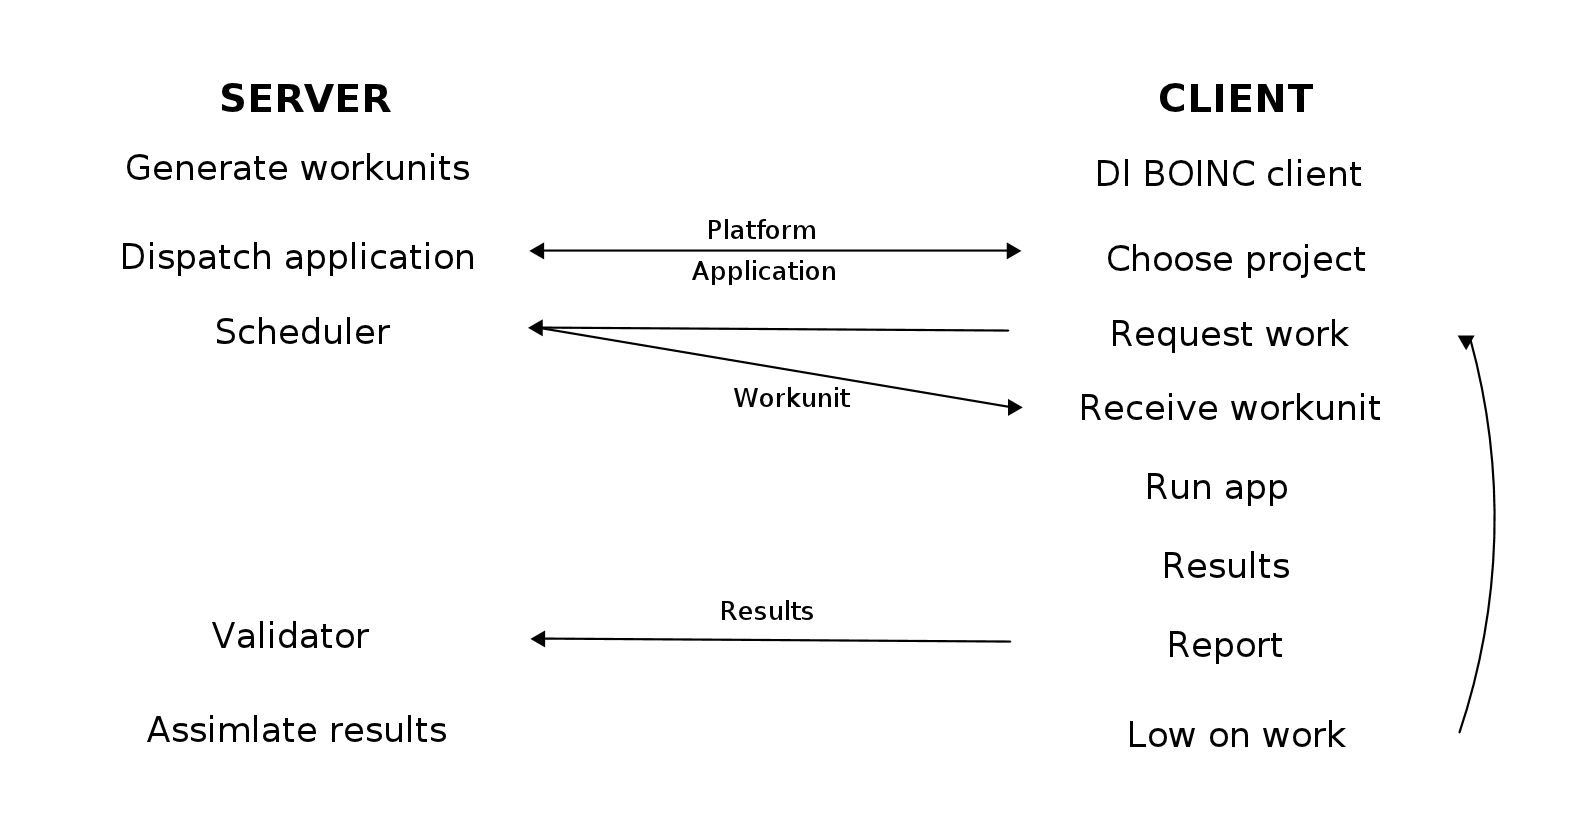
\includegraphics[width=14cm]{images/workflow}

\caption{Example workflow}
\end{figure}

\subsection{Grid-enabling a simple BOINC project}
A scientist attempting to turn an existing application into a volunteer computing project must  determine how the application will be parallelised, modify his existing application to make use of the BOINC API and finally provide the server-side deamons responsible for scheduling,  generating new workunits and validating and assimilating incoming results.
The first of these tasks, parrellelising the computation is highly application specific and has little to do with the structure and components of a BOINC project but it may be insightful to give further consideration to the BOINC API and the various deamons running on the server.
\subsubsection{The BOINC API}
The BOINC API provides a set of functions that firstly allow the client and the application to communicate and secondly improves portability of the application between different platforms.
An application must notify the client when it initialises through a call to \texttt{boincinit()} and return a value when terminating so that the client may track whether the computation was successful or not. 
The API also handles input and output, resolving logical names to actual filenames as specified in the workunit and providing wrappers for functions which execute differently on different platforms, for example a \texttt{boincfopen()} function which replaces the standard fopen call for opening functions so that on Windows hosts, where files may become temporarily locked, the function attempts to open the file multiple times within short succession and on Unix, where fopen() occasionally fails with a specific error code, it check for this error code and retries accordingly. 
\emph{Checkpointing}, or saving the current state of the computation in such a way that the computation may be resumed from that point, is very important in volunteer computing as there is no way of knowing when a host may be turned off or fail. Applications may choose their own minimum time between checkpoints, usually based on how long it takes to checkpoint, and may repeatedly call the method \emph{boinctimetocheckpoint()} to determine when to checkpoint. Checkpointing is also an example of a \emph{critical section} of an application, or a section which may not be interrupted by the client. 
BOINC  allows communication between the appliication and server through \emph{trickle messages}, small messages that are sent up from the client or down from the server and which has a very high priority. A trickle down message may for example be sent to notify an application that the result which it is computing is no longer needed and should be aborted, similarly a trickle-up message may be sent to the server to notify it that although a results has reached its deadline it is still being sunccessfully computed, in which case the original deadline should be extended.
The remainder of the API mainly focusses on providing methods which let the client register the time that the computation takes and monitor its progress, the full API along with a brief summary of every function as described in \cite{boincwiki, boincgit} may be found in Table \ref{tab:api}.
\begin{table} 
\caption{A selection of the parameters that may be specified in the output template, as found in \cite{boincwiki}}
\begin{tabular}{lp{11.6cm}}\toprule
 \multicolumn{2}{l}{\textbf{Output template options} \cite{boincwiki}   }\\ \cmidrule(r){1-2}
 \verb|name| & The physical file name of the output file\\
\verb|open_name| & The "logical name" by which the application will reference the file.\\
\verb|max_nbytes| & Maximum file size. If the actual size exceeds this, the file will not be uploaded, and the job will be marked as an error.\\
\verb|url| & the URL of the file upload handler. \\ 
\verb|no_delete| & If present, the file will not be deleted on the server even after the job is finished.\\
\verb|report_immediately| & If present, clients will report this job immediately after the output files are uploaded, otherwise they may wait up to a day. 
\\  \bottomrule
\end{tabular}\label{tab:api}
\end{table}
 
\subsubsection{Deamons}
The main task of the work generator is inserting new workunits or jobs into the project database. This may happen once, at the start of the project, in a number of discrete batches or continuously as results are returned from the volunteers. It is also possible to develop a web interface which allows for the remote submission of jobs.
Before implementing the work generator, however, projects must decide on templates for the workunits and results. These templates are XML files which provide  the application with the necessary information to compute the workunit and are typically re-used for millions of jobs. 
An input template may for example specify the name of the actual file to which the logical filename must be resolved, possible command-line arguments along with workunit attributes such as an estimate of its execution time, the resources required for the computation and the deadline by which the server expects to receive the result before re-issuing the workunit to a different host.  
Similarly, the output template defines the number of files returned to the server and where they are to be found or generated, a selection of the most important options that may be specified in the input and output templates may be found in Tables \ref{tab:intemplate} and \ref{tab:outtemplate}, respectively. The work generator ensures that the required files and templates are available before entering the workunit into the database. The BOINC API provides both a command-line tool and  a C/C++ method which inserts new jobs into the project database.
\begin{table} 
\caption{A selection of the parameters that may be specified in the input template, as found in \cite{boincwiki} }
\begin{tabular}{lp{11.5cm}}\toprule
\multicolumn{2}{l}{\textbf{Input template options }\cite{boincwiki} }\\ \cmidrule(r){1-2}
\verb|open_name| & The logical name of the file used in the application, \emph{e.g. `in'}.\\
\verb|command_line| & The command-line arguments to be passed to the main  application.  \\
\verb|rsc_fpops_est| &
An estimate of the number of floating-point operations required to complete the job, used to estimate how long the job will take on a given host.\\
\verb|rsc_fpops_bound| &
An upper bound on the number of floating-point operations required to complete the job. If this bound is exceeded, the job will be aborted.\\
\verb|rsc_memory_bound| &
An estimate of job's largest working set size. The job will only be sent to hosts with at least this much available RAM. If this bound is exceeded, the job will be aborted.
\\
\verb|rsc_disk_bound| &
A bound on the maximum disk space used by the job, including all input, temporary, and output files. The job will only be sent to hosts with at least this much available disk space. If this bound is exceeded, the job will be aborted.\\
\verb|rsc_bandwidth_bound| &
If nonzero, this job will be sent only to hosts with at least this much download bandwidth. Mainly used for jobs with very large input files. \\
\verb|delay_bound| &An upper bound on the time (in seconds) between sending a result to a client and receiving a reply.  If the client doesn't respond within this interval, the server 'gives up' on the result and generates a new result, to be assigned to another client.  
\\
\verb|min_quorum| &
The minimum size of a quorum. The validator is run when there are this many successful results. If a strict majority agree, they are considered correct. Set this to two or more if you want redundant computing.
\\
\verb|target_nresults| &
How many results to create initially. This must be at least \verb|min_quorum|. It may be more, to reflect the ratio of result loss, or to get a quorum more quickly.
\\
\verb|max_error_results| &
If the number of client error results exceeds this, the work unit is declared to have an error; no further results are issued, and the assimilator is triggered. This safeguards against workunits that cause the application to crash.
\\
\verb|max_total_results| & If the total number of results for this workunit would exceed this, the workunit is declared to be in error. This safeguards against workunits that are never reported (\emph{e.g.} because they crash the core client).
\\
\verb|max_success_results| & If the number of success results for this workunit exceeds this, and a consensus has not been reached, the workunit is declared to be in error. This safeguards against workunits that produce non-deterministic results.
\\
\verb|priority| &  Higher-priority work is dispatched first \\
\verb|size_class| & Used to define workunits of different sizes, for example in the case where the GPU version of an application is orders of magnitudes faster than the CPU version. \\ \bottomrule
\end{tabular} \label{tab:intemplate}
\end{table}

\begin{table} 
\caption{A selection of the parameters that may be specified in the output template, as found in \cite{boincwiki}}
\begin{tabular}{lp{11.6cm}}\toprule
 \multicolumn{2}{l}{\textbf{Output template options} \cite{boincwiki}   }\\ \cmidrule(r){1-2}
 \verb|name| & The physical file name of the output file\\
\verb|open_name| & The "logical name" by which the application will reference the file.\\
\verb|max_nbytes| & Maximum file size. If the actual size exceeds this, the file will not be uploaded, and the job will be marked as an error.\\
\verb|url| & the URL of the file upload handler. \\ 
\verb|no_delete| & If present, the file will not be deleted on the server even after the job is finished.\\
\verb|report_immediately| & If present, clients will report this job immediately after the output files are uploaded, otherwise they may wait up to a day. 
\\  \bottomrule
\end{tabular}\label{tab:outtemplate}
\end{table}

It is highly likely that a new project will, at least initially, make use of the default scheduler  provided along  with the BOINC source code.
The scheduler is responsible for accepting requests for work from hosts, assigning work to hosts based on a combination of their available resources, the estimated execution time of the available workunits and the historical accuracy of a host. Larger workunits are thus sent to hosts who historically return less erroneous computations and have more resources available in order to minimise the expected computation time that will be lost if a host returns an error after an extended period of   work.
Secondary objectives which may be included in the scheduler is finishing a specific batch of workunits as soon as possible or limiting the number of workunits that a host may receive on a single day to prevent hosts from repeatedly returning the same results and claiming credit for them.

The main task of the validator is to compare results for correctness. Care must be taken when comparing results from different platforms, for example, the end-of-line character is different between Windows and Linux making a character by character comparison of the output files impossible. If an application does a lot of floating-point operations projects may elect to enforce a measure called \emph{homogeneous redundancy} to ensure that results from the same workunit are assigned to identical platforms, alternatively fuzzy" comparisons may be made by comparing floating-point numbers with a degree of tolerance. A measure called \emph{adaptive replication} may also be used, which decides on the number of replications of a specific workunit based on the historical error rate of the host which was assigned the first result, if the host usually returns accurate results the probability of replication taking place for that workunit will be small.
Validation takes place by majority when a quorum of results have been received and marks a result, along with its associated output files, as the canonical result against which any other results of the same workunit are compared in order to determine whether it was computed successfully and deserves credit.
Two sample validators are provided with the BOINC source code, the first is mainly used for testing purposes and simply marks every received result as successful while the second does a bitwise comparison of output files.

Once results are verified they should be marked accordingly in the database so that they are not assigned to any further hosts, their input files may be deleted from the location where they were accessible to hosts and the canonical output files may be moved to a specific location.
The sample assimilator does exactly this and it is up to projects to decide what other post-processing tasks to perform on validated results.

Projects which make use of trickle messages must also provide a deamon to handle these messages. Trickle messages may for example be used by the application to periodically send its current computation state to the server  so that the server may   determine whether to assign partial credit for the work done up to the current point  or   to abort the computation based on some internal logic.

\subsection{Special types of applications}
In addition to the basic functionality BOINC allows applications to display graphics, execute on multiple cores or GPUs through OpenCL \cite{opencl}, and CUDA \cite{cuda} or even run entirely within a virtual machine. 
\subsubsection{Graphics applications}
Publicly-launched volunteer computing projects usually attempt to provide volunteers with some visualisation of the computation running on their machine, either as a screensaver or in a window which can be opened in the BOINC Client Manager. The main reason for providing graphics is to further engage the public in the goals and workings of a scientific project in order to increase involvement, examples of graphics provided by SETI@Home and WCG may be seen in Figure \ref{fig:boincgraphics}.
\begin{figure}[htb]\label{fig:boincgraphics}
\centering
\begin{minipage}{7.5cm}
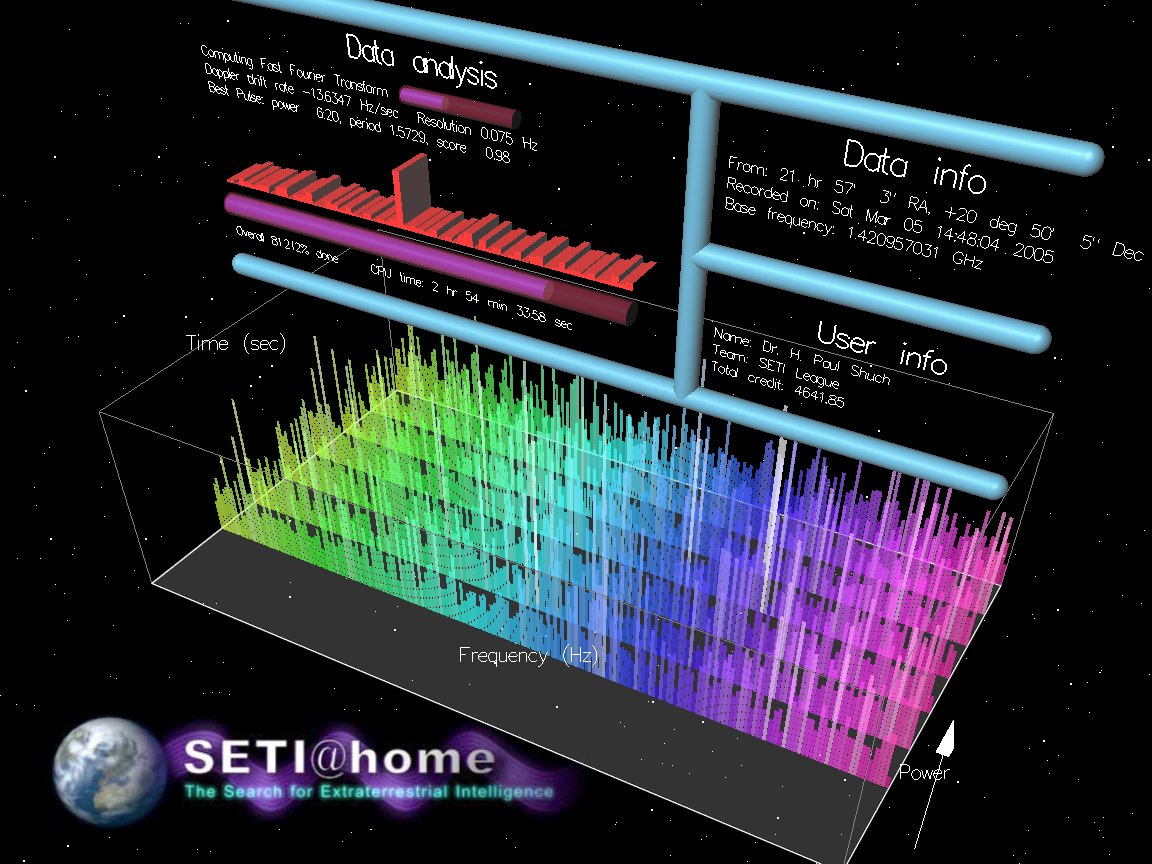
\includegraphics[width=7.5cm]{images/graphics1}
 \end{minipage} \hspace{.1cm}
\begin{minipage}{7.5cm}
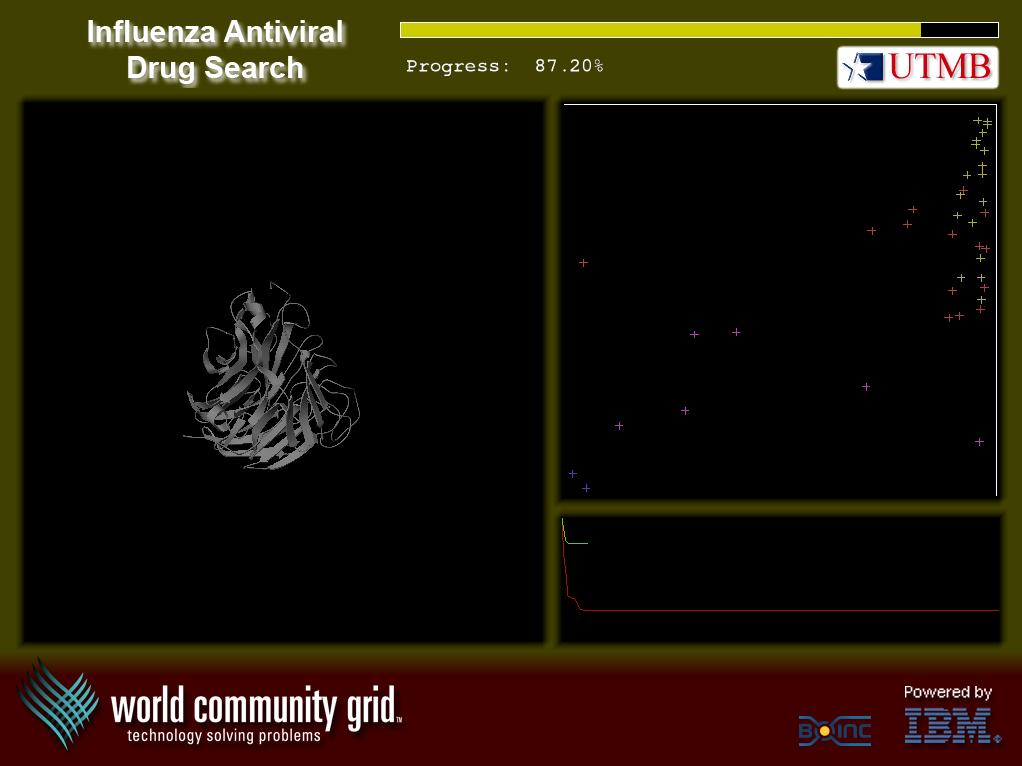
\includegraphics[width=7.5cm]{images/graphics2}
 \end{minipage}
\caption{Graphical applications provided by SETI@Home and WCG provide volunteers with an indication of the state of the current computation}
\end{figure}
  In a  recent survey of XXXX volunteers by IBM's World Community Grid project \cite{wcg}, however, XX\% of volunteers said that the graphics play a role in their involvement in a project \cite{wcg2013}, thereby casting some doubt on the actual benefit of graphical applications. Graphics applications are usually separate from the main scientific application, built on  a specific  BOINC graphics library and makes use of OpenGL \cite{opengl} for displaying graphics. Communication with the main application takes place through shared memory, the main application would periodically store a representation of its current state and progress in  a block of memory which is accessible to the graphics application, from where it will be read and displayed. Graphics applications can also display static images, text or web-based graphics by opening a browser windows pointing to a specific URL.

\subsubsection{Muti-core and GPU applications}
CPU manufacturers have been dealing with the limit placed on CPU frequency by increasing the number of cores provided and it seems that this trend will continue for some time. In cases where the completion time of individual workunits want to be increased, or the memory footprint of the application is too large to allow a separate copy of the application to run on every core it may be desirable to have a multi-threaded application developed in OpenCL, MPI, OpenMP, CUDA or a number of other languages. BOINC also supports what it calls `coprocessors' or GPUs designed by NVIDIA, AMD or Intel. Available GPUs are reported to the scheduler by the BOINC client, which also keeps track of which instances on every GPU is currently allocated. To prevent system, failures GPU kernels are  executed within critical sections, which may not be killed by the BOINC client and  BOINC projects may define workunits of different size classes to compensate for the potentially dramatic difference in speed between CPU and GPU versions of the same applications adnd thereby ensure that a typical workunit will take approximately the same amount of time irrespective of the architecture on which it is executed.

\subsubsection{Applications which run inside virtual machines}
BOINC supports application which run entirely within virtual machines. This approach has two distinct advantages in that it provides the highest level of security for the host machine, as virtual machines cannot access or modify the host system and there is no need to build applications for different architectures as every application will run on a virtual computer with exactly the same runtime environment on any platform.  
There are however also some additional complexities which arise from using applications inside virtual machines such as the fact  that hosts require software such VirtualBox to mount the machine image, yet VirtualBox  is not currently available for all processors. GPU applications can not currently be run inside VirtualBox and not all processors are capable of running both 32- and 64-bit virtual machines, so images of both will have to be provided. Distributing the virtual machine image also increases the size of the first download to approximately 200Mb, which may be prohibitive for volunteers with limited bandwidth.

\subsection{Setting up a server and project maintenance}
As stated in \S \ref{}, a BOINC project consists mainly of a MySQL database, a directory structure and a configuration file which specifies the options, deamons and periodic tasks which must be performed and as such, it is possible to use almost any computer as a  BOINC server \cite{boincwiki}.

As with any server reliability and security is of the utmost importance, a server should at least be placed behind a firewall and have a reliable internet connection for connecting with volunteers, with a static IP address. Additional hardware measures which may  be taken to improve reliability  include an uninterrupted power supply, automatic backups adequate cooling and hot-swappable spares. Any Unix or Linux distribution may be used for setting up a server and  detailed instructions are available at \cite{boincwiki}. 
Alternatively a project may elect to host its server either on the Amazon Elastic Cloud Computing (EC2) service, which removes   potential concerns about hardware reliability and security, or host in within a virtual machine. A virtual machine image is available which has all the software packages required to set up a server, as well  as a number of installing and configuration scripts.  

Once a server has been set up a number of maintenance tasks must be performed regularly, \emph{e.g.} reviewing the deamon logs for errors, deleting files as they are no longer needed and archiving  and purging old jobs from the database to prevent the database from becoming to large. BOINC provides small programmes for all of these activities. Additionally it is possible that, due to the popularity of a project, a server may no longer be able to keep up with  the traffic generated by the volunteers, which will result in dropped connections, slow website access, deamons which fall behind and very slow database queries. A number of strategies are discussed in the BOINC documentation for upgrading the server in such scenarios, including upgrading the server hardware,  hosting the database on a separate server and  parallelising the deamons and scheduler so that multiple instances are constantly running.

\subsection{Security}
According to \cite{boincwiki} a number of security concerns arise from the inherently public nature of volunteer computing, chief amongst which are
\begin{itemize}
\item result falsification,
\item credit falsification,
\item denial-of-server attacks on the project servers, 
\item theft of project files or participant account information, including email addresses, and
\item the distribution of malicious executables.
\end{itemize}
Result and credit falsification may be limited b y making use of replication and validation and limiting the number of results a user may receive creit for in a single day. 
BOINC protects projects agains denial-of-service attacks, in which servers are overrun by requests and transfers from automated programs, by providing a size limit for every file that is uploaded to the server (refer to Table \ref{tab:outtemplate} in \S \ref{}) and making use upload certificates. Every project is responsible for protecting its own users' account information against theft and servers should be subjected to regular security audits. Successful attacks of this type has harmed the image of specific projects and volunteer computing in general very much. \cite{son}
The greatest security risk to volunteer computing project is the potential that a server may be broken into and used to distribute malicious executables to volunteers. In order to prevent this a code-signing software is used which signs every approved and secure application version as authenticate. The computer which is responsible for code-signing applications should be kept in `cold storage', in other words, physically secure and completely disconnected from the network to prevent attackers from breaking into it and authenticating their applications. 

\subsection{Challenges}
Decline in recent years, trouble breaking out of the core demographic of technically minded males. New initiatives such as cycles for change make use of social media platforms to engage a wider audience, indeed cycels for change boast an even number of male and female users. Also largely unexploited in Cihine, little hardware, hardware is not standardised, etc, languages.

\subsection{Basic workflow}

 
Specifics about rgidenabling, splitting up the search tree,  checkpointing, validating, workgenerations, handling inconsistent subtree sizes.1


\section{challenges}
demographics: 92\% male in \cite{anderson:pc}



\section{Chapter summary}
\chapter{Deployment of the distributed enumeration project}
% put these two lines after every \chapter{} command
\vspace{-2em}
\minitoc

Chapter 5 will contain details pertaining to the method of deploying a small-scale distributed search based on the design set out in Chapter 4 as a proof of concept.  It will include how awareness of the project was raised in the scientific community, the  challenges involved in launching the project as well as the lessons learnt for the possible future deployment of larger scale projects.  The chapter will conclude with the results of the distributed computing project designed in Chapter 4, most likely the enumeration of main classes of MOLS of order 8 or 9.  It will also give a summary of the distributed enumeration in terms of number of volunteers, locality, how work was done by each of the volunteers etc. 

\section{Methodology}

\subsection{Technical specifications}
\subsection{Raising public awareness}
\subsection{Challenges}

s\\
\section{Distributed enumeration of MOLS}
\subsection{Enumeration summary}
\subsection{Results}

\section{Chapter summary}
\input{Ch6_Feasibility}
\chapter{Conclusions}
% put these two lines after every \chapter{} command
\vspace{-2em}
\minitoc

The final chapter summarizes the work in this thesis, briefly recount the contents of each preceding chapter and proceeds to evaluate the contributions made.  The thesis concludes with a reflection on possible continued studies arising from the contributions made by the thesis.

\section{Overview of work}

\section{Summary of contributions}

\section{Possible further work}
%Appendices
\appendix
\chapter{Group theory} \label{App_group}
group, quasi group, loop
Cayley table
complete mapping

%%%%%%%%%%%%%%%%%%%%%%%%%%%%%%%%%%%%%%%%%%%%%%%%%
%
% start writing
%
%%%%%%%%%%%%%%%%%%%%%%%%%%%%%%%%%%%%%%%%%%%%%%%%


\chapter{Introduction}
% put these two lines after every \chapter{} command
\vspace{-2em}
\minitoc
this is a chapter.
\startarabicpagenumbering % must be just after the first \chapter{} command



%%%%%%%%%%%%%%%%%%%%%%%%%%%%%%%%%%%%%%%%%%%%%%%%%
%
% some tips on creating nice tables
%
%%%%%%%%%%%%%%%%%%%%%%%%%%%%%%%%%%%%%%%%%%%%%%%%
\chapter{Tables}

% TABLE SHADING
%===============
%
% uncomment to change the default shades (gray!45 and gray!25) for the tables in your thesis:
%    \colorlet{tableheadcolor}{gray!45}  % headers
%    \colorlet{tablerowcolor}{gray!25}   % normal rows
%
% \headcol                 - for shading the header of your table
% \rowcol                  - shades an entire row
% \rowcolor{color}         - for custum coloring of a row
%
% \cellcolrow              - shades a single entry in the table the shade of a row
% \cellcolhead             - shades a single entry in the table the shade of the header
% \cellcolor{color}        - for custom colouring of a single entry in the table
%
% \rowcolors{startrow}{oddrowcolor}{evenrowcolor} - for automatic shading of rows, put in table environment
%   examples:
%     \rowcolors{3}{gray!25}{} - shades 3rd row and every second row after that
%     \rowcolors{2}{}{gray!25} - shades 2rd row and every second row after that




% TABLE LINES
%=============
%
% \toprule     - the top-most line of a table, does not work with shading
% \hline       - normal line, does not work with shading
% \midline     - normal line, does not work with shading
% \bottomrule  - a line for the bottom of the table, does not work with shading
%
% \topline     - the top-most line of a table if the header is shaded
%
% \midline     - the line between the headings and the table body
% \midlinecbw  - a line for when the previous row is rowcolor and the next line is white
% \midlinecw   - a line with no black, to further separate a rowcolor row and a white row
% \midlinewbc  - a line for when the upper row is white and the next line is rowcolor
% \midlinewc   - a line with no black, to further separate a white row and a rowcolor row
%
% \bottomline  - a line for the bottom of the table, when the last row is white
% \bottomlinec - a line for the bottom of the table, when the last row is rowcolor




% EXAMPLE
%========

\begin{table}[h!tb]

\centering

\rowcolors{3}{gray!25}{}

\begin{tabular}{ccc}\topline
\headcol       & & \\ \midline
\hspace{5cm} \ & & \\
               & & \\ 
               & & \\ 
               & & \\ 
               & & \\ 
               & & \\ \bottomlinec
\end{tabular}

\caption[Example 1 as in list of tables]{Example 1}
\label{ex1}

\end{table}




% EXAMPLE
%=========
%
% example using multicolumn, multirow and the sideways environment

\begin{table}[h!tb]

\centering

\begin{tabular}{cc|rrrrrr}\hline

&&\multicolumn{6}{c}{this goes across 6 columns}\\

 && col a & col b & col c & col d & col e & col f \\ \hline \hline

\multirow{6}{*}{
%
\begin{sideways}
this is sideways,
\end{sideways}
%
\begin{sideways}
and goes across
\end{sideways}
%
\begin{sideways}
six rows
\end{sideways}
%
}

& row 1 \\
& row 2 \\
& row 3 \\
& row 4 \\
& row 5 \\
& row 6 \\ \hline

\end{tabular}

\caption[Example 2 as in list of tables]{Example 2}
\label{ex2}

\end{table}




%%%%%%%%%%%%%%%%%%%%%%%%%%%%%%%%%%%%%%%%%%%%%%%%%
%
% figures - nothing too special here 
%
%%%%%%%%%%%%%%%%%%%%%%%%%%%%%%%%%%%%%%%%%%%%%%%%
\chapter{Figures}


% BASIC EXAMPLE
%================

\begin{figure}[h!tb]
\centering

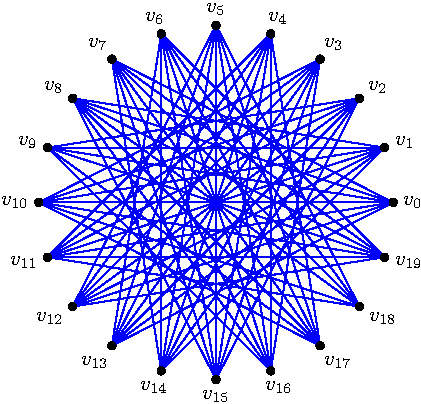
\includegraphics{figure} % not necessary to give extension - now you can shift between compiling to ps or to pdf without any problems
 
\caption[Figure caption in list of figures]{An example of the figure environment}

\end{figure}





\newpage





% SUBFIG EXAMPLE
%================
%
% usage: \subfloat[][caption]{...figure code...\label{label}}

The subfigures are Figures \subref{firstfigure}, \subref{secondfigure}, \subref{thirdfigure} and \subref{fourthfigure}.

\begin{figure}
\centering

\subfloat[][First subcaption.]{
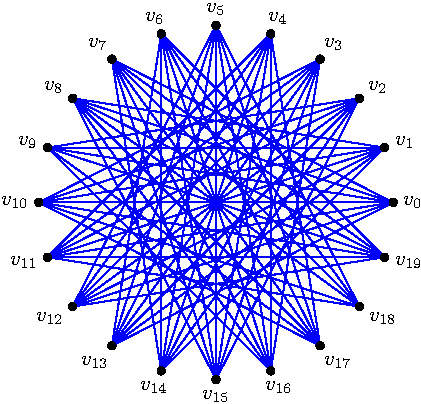
\includegraphics{figure}
\label{firstfigure}
}
\quad
\subfloat[][Second subcaption]{
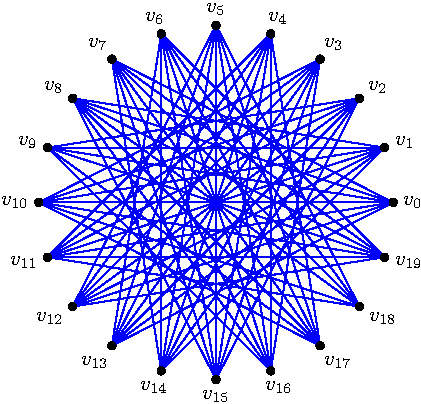
\includegraphics{figure}
\label{secondfigure}
}
\\
\subfloat[][Third subcaption]{
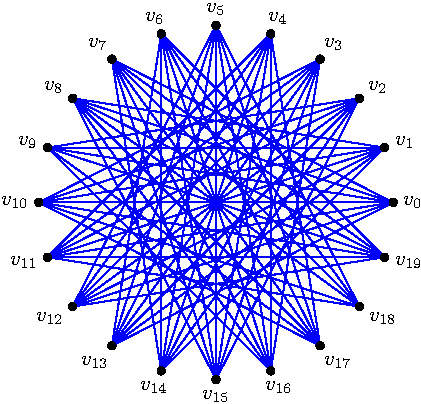
\includegraphics{figure}
\label{thirdfigure}
}
\quad
\subfloat[][Fourth subcaption]{
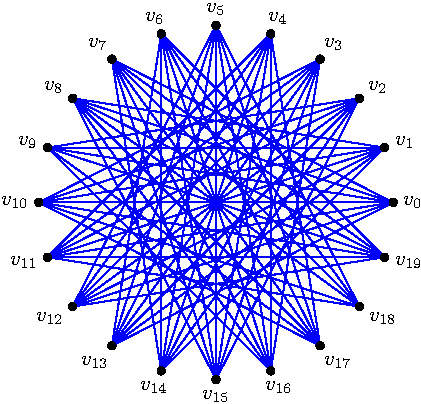
\includegraphics{figure}
\label{fourthfigure}
}
\caption{How to use the {\sf subfig} package.}
\label{thislabel}
\end{figure}


%%%%%%%%%%%%%%%%%%%%%%%%%%%%%%%%%%%%%%%%%%%%%%%%%
%
% how to typeset algorithms
%
%%%%%%%%%%%%%%%%%%%%%%%%%%%%%%%%%%%%%%%%%%%%%%%%
\chapter{Algorithms}

% USE THE TEMPLATE BELOW FOR YOUR ALGORITHMS
%============================================
%
% \begin{algorithm}
% 
% \SetKwInOut{Input}{Input}
% \SetKwInOut{Output}{Output}
% 
% \Indm
% \Input{Description of the input to the algorithm.}
% \Output{Description of the output from the algorithm.}
% \Indp
% 
% \BlankLine
% 
%   % main algorithm code here
% 
% \caption{Algorithm example}
% \label{alg}
%
% \end{algorithm}



\begin{algorithm}

\SetKwInOut{Input}{Input}
\SetKwInOut{Output}{Output}

\SetKwData{Left}{left}
\SetKwData{This}{this}
\SetKwData{Up}{up}
\SetKwFunction{Union}{Union}
\SetKwFunction{FindCompress}{FindCompress}

\Indm
\Input{Description of the input to the algorithm.}
\Output{Description of the output from the algorithm.}
\Indp

\BlankLine

\emph{special treatment of the first line}\;
\For{$i\leftarrow 2$ \KwTo $l$}{
  \emph{special treatment of the first element of line $i$}\;
  \For{$j\leftarrow 2$ \KwTo $w$}{\label{forins}
    \Left$\leftarrow$ \FindCompress{$Im[i,j-1]$}\;
    \Up$\leftarrow$ \FindCompress{$Im[i-1,]$}\;
    \This$\leftarrow$ \FindCompress{$Im[i,j]$}\;
    \If(\tcp*[h]{O(\Left,\This)==1}){\Left compatible with \This}{\label{lt}
      \lIf{\Left $<$ \This}{\Union{\Left,\This}}\;
      \lElse{\Union{\This,\Left}\;}
    }
    \If(\tcp*[f]{O(\Up,\This)==1}){\Up compatible with \This}{\label{ut}
      \lIf{\Up $<$ \This}{\Union{\Up,\This}}\;
      \tcp{\This is put under \Up to keep tree as flat as possible}\label{cmt}
      \lElse{\Union{\This,\Up}}\tcp*[r]{\This linked to \Up}\label{lelse}
    }
  }
  \lForEach{element $e$ of the line $i$}{\FindCompress{p}}
}

\caption[Algorithm caption as in list of algorithms]{Algorithm example}
\label{alg}

\end{algorithm}



%%%%%%%%%%%%%%%%%%






%%%%%%%%%%%%%%%%%%
%
% bibliography
%
%%%%%%%%%%%%%%%%%%

\cite{*} % cites all items in your .bib file for the purpose of testing biblatex - REMOVE!

\printbibliography[heading=bibintoc] % prints a bibliography containing all (and only) cited items

%%%%%%%%%%%%%%%%%%

\end{document}
